\clearpage
\setcounter{page}{1}
\maketitlesupplementary

\section{More Related Works}
\label{sec:more_related_work}

% This supplementary section reviews the technological evolution of video generation and embodied world models. We focus specifically on the architectural paradigms—Autoregressive Transformers and Diffusion Models—that have paved the way for modern, physics-consistent world simulators.

\paragraph{Video Generation Models.}
The quest for scalable video synthesis has converged on two dominant architectures, both serving as backbones for predictive world modeling.

\textbf{Autoregressive Transformers.} 
Inspired by Large Language Models, architectures like VideoGPT~\cite{yan2021videogpt} treat video generation as a discrete sequence modeling task. By tokenizing frames via VQ-VAE~\cite{van2017neural}, these models predict visual token sequence-by-sequence. This paradigm, akin to next-word prediction, naturally aligns with the state-transition logic of world models. Notable examples like Genie~\cite{bruce2024genie} utilize this spatiotemporal autoregressive objective to build interactive environments and predictive models from diverse video data. However, the discrete quantization often imposes an upper bound on visual fidelity, resulting in the loss of high-frequency details.

\textbf{The Diffusion Paradigm.} 
Diffusion Models (DMs) have established a new state-of-the-art by formulating generation as iterative denoising. Early attempts like SVD~\cite{blattmann2023stable} adapted 2D U-Nets with temporal layers, excelling at texture but often treating time as a secondary dimension. The recent shift to Diffusion Transformers (DiT)~\cite{peebles2023scalable}, exemplified by Wan~\cite{wan2025wan}, Cosmos~\cite{cosmos2}, Sora~\cite{sora2024}, operates on unified spacetime patches. These models demonstrate emergent capabilities akin to a physics engine—simulating fluid dynamics and occlusion—making them ideal candidates for high-fidelity world simulation.


\paragraph{Embodied World Models.}
Unlike passive video generation, embodied world models function as predictive engines ($s_{t+1} | s_t, a_t$) to facilitate agent planning.

\textbf{From Latent States to Pixel Space.} 
Early research balanced between efficiency and detail. The Dreamer series~\citep{hafner2023mastering} prioritized computational tractability by learning dynamics in a compact latent space, enabling efficient RL planning but producing schematic visual reconstructions. Conversely, pixel-space approaches like RoboNet~\citep{dasari2019robonet} predicted future frames directly from interaction logs. While capturing texture, these models often struggled with the stochastic nature of real-world physics, leading to blurry predictions over long horizons.

\textbf{Generalist Simulators.} 
Recent efforts converge generative AI with robotics to create "Generalist Simulators." Foundation models like UniSim~\citep{yang2023unisim} and GAIA-1~\citep{hu2023gaia} leverage internet-scale data to learn high-level physics for zero-shot generalization. 
% Furthermore, to address the geometric limitations of 2D video, frameworks like 3D-VLA~\citep{zhen20243d} and PhysGaussian~\citep{xie2024physgaussian} integrate explicit 3D representations (e.g., point clouds, Gaussians) into the prediction loop, allowing the world model to reason explicitly about depth and collision.


\section{Models Detail}
Since the models have different versions and parameter sizes, and also generate videos of different durations and resolutions, we introduce the models we use, their specific versions and parameter counts, as well as the generated durations and resolutions, to facilitate comparison and reproduction.
\paragraph{Kling.~\cite{Kling}}
A large-scale diffusion-transformer video generator known for photorealistic long-form outputs, strong motion control, and realistic physics. It employs a latent-space DiT architecture with 3D VAE compression and is optimized for high-consistency content such as sports or human motion. We used the latest Klingv2.1 to generate a 5-second 720p video.

\paragraph{Hailuo.~\cite{Hailuo}}
Hailuo is a commercial text-to-video and image-to-video model designed for high-quality short-form generation (6–10 seconds, up to 1080p). It emphasizes photorealism, smooth motion, and subject consistency, making it a strong closed-source baseline for perceptual quality. We use the publicly accessible Hailuo-02 for 5-second 768p video generation and evaluation.

\paragraph{CogVideoX.~\cite{yang2024cogvideox}}
An open diffusion-transformer video generator available in 2B/5B variants. It can produce ~10-second clips with improved motion expressiveness using a 3D causal VAE and MoE-style transformer backbone. The model supports both text-to-video and image-to-video generation and serves as a strong open-source baseline for long-duration video synthesis. For evaluation, we use CogVideoX-I2V-5B to generate 5-second 1360x768 videos.

\paragraph{Cosmos-Predict.~\cite{agarwal2025cosmos,cosmos2}}
NVIDIA’s open-source world-model family for video-based state prediction. It supports Text-/Image-/Video-to-World forecasting and can generate long-horizon, physics-aware video rollouts. The model is trained on large-scale real-world videos and emphasizes dynamics, object permanence, and 3D geometry consistency. We evaluate both Cosmos-Predict1 and the stronger Cosmos-Predict2 variants. Both Predict1\&2 are 5-second 720p, but the parameters of the model are 7B and 2B, respectively.

\paragraph{Wan.~\cite{wan2025wan}}
Wan is a series of open-source Diffusion Transformer video models (e.g., Wan 2.1/2.2) trained on large-scale image–video corpora. They support text-to-video and image-to-video generation, producing 5–10 second clips with strong spatial–temporal coherence. Wan models use 3D VAE compression and DiT backbones to improve motion consistency and are widely used as high-quality open video generation baselines. We fix the resolution for a 5-second 832x480 generation with Wan2.1-I2V-14B.

\paragraph{WoW.~\cite{chi2025wow}}
WoW is a 14B-parameter open-source embodied world model designed for physically grounded video prediction in robotic manipulation. It generates future video rollouts conditioned on visual observations and task instructions, with inductive biases (e.g., DINOv2 token distillation) that encourage spatial and physical consistency. Unlike generic video models, WoW explicitly targets planning, contact dynamics, and multi-step task execution. We use the different backbones of WoW, including Wan, Cosmos-Predict1, and Cosmos-Predict2, for evaluation; all generated video settings are the same as the backbone models.

\section{Detailed Metrics}
\label{sec:more_metrics}
\begin{figure*}[!h]
  \centering
  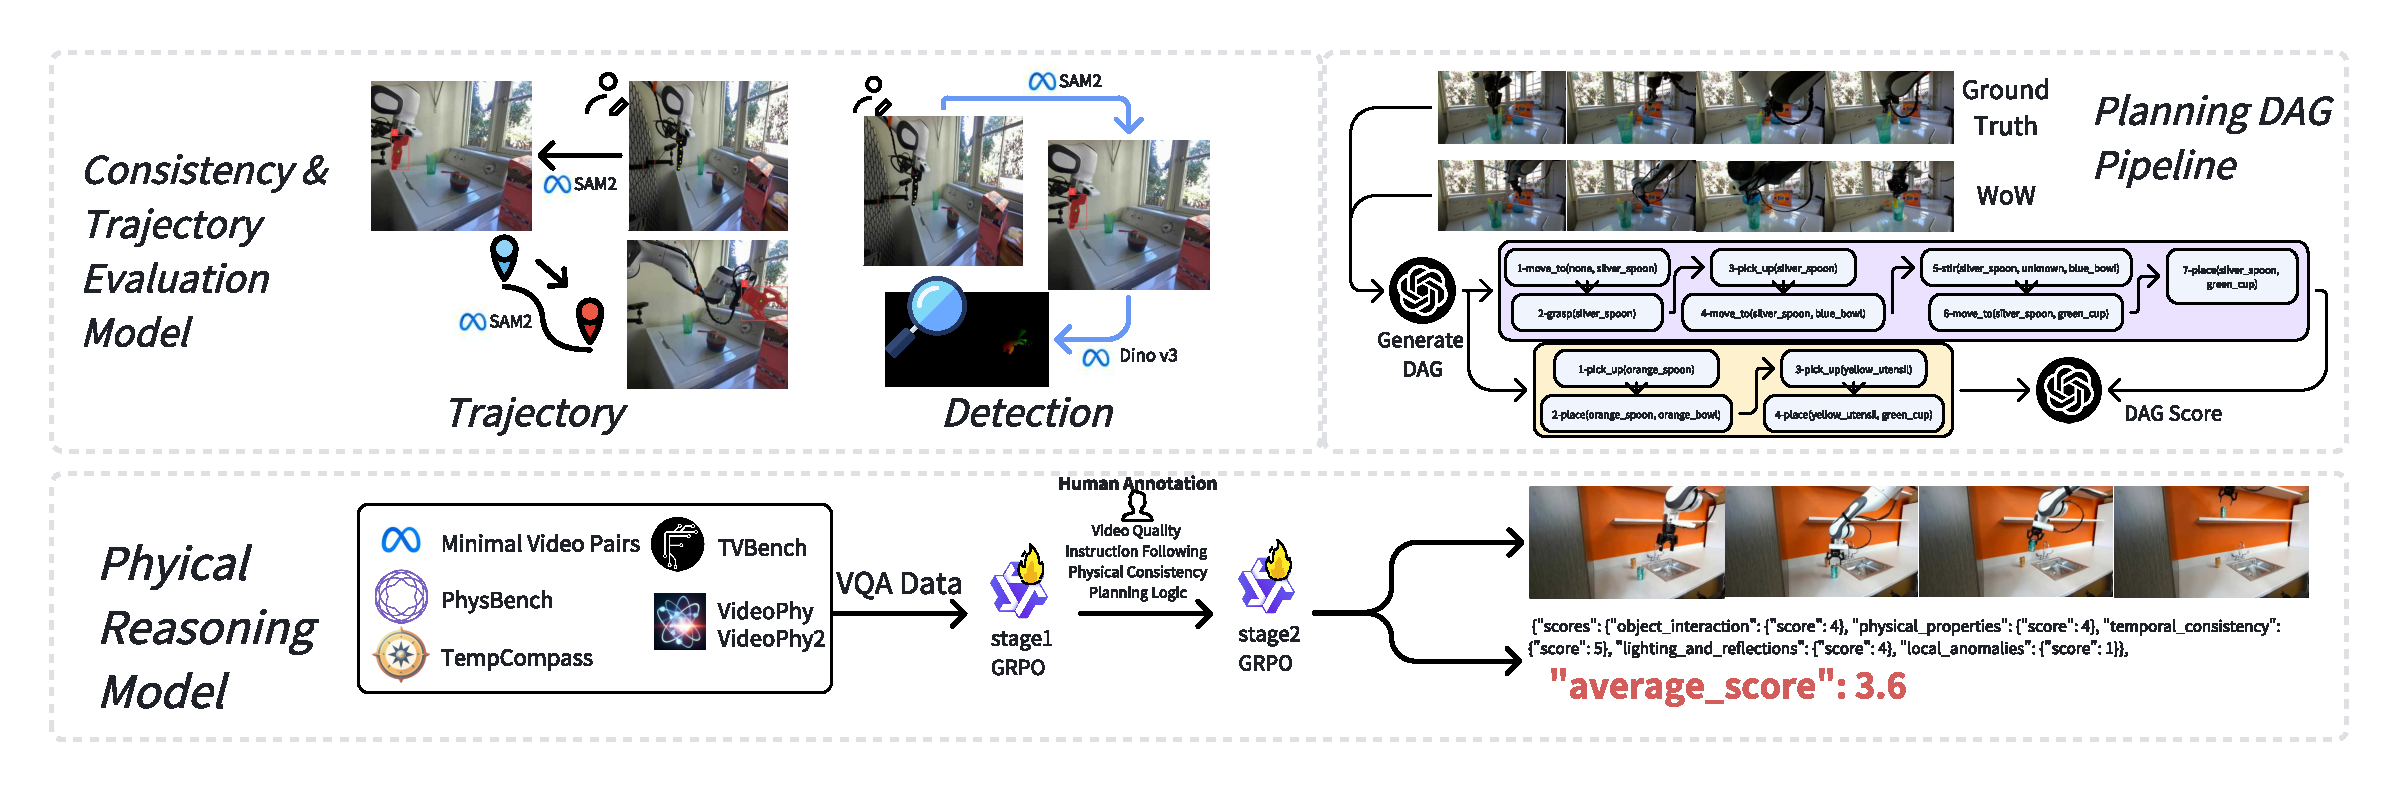
\includegraphics[width=1.0\textwidth]{figs/metric.pdf} 
  \caption{\textbf{Overview of WoW-World-Eval Metrics.} }
  \label{fig:metric}
\end{figure*}

\subsection{Visual Fidelity.}
To evaluate the visual fidelity of generated videos, we adopt a suite of complementary metrics that capture low-level reconstruction accuracy, perceptual similarity, and distributional realism. These include 
FVD, SSIM, PSNR, DINO, and DreamSim.

\paragraph{Fréchet Video Distance (FVD).}
FVD is a distribution-level metric that measures how closely generated video features match those of real videos. 
Given feature means and covariances $(\mu_r, \Sigma_r)$ for real videos and $(\mu_g, \Sigma_g)$ for generated videos extracted using an I3D network, FVD is defined as:
\[
\mathrm{FVD}
= \|\mu_r - \mu_g\|_2^2
+ \mathrm{Tr}\!\left(\Sigma_r + \Sigma_g 
- 2\left(\Sigma_r\Sigma_g\right)^{1/2}\right).
\]
Lower FVD indicates higher spatial-temporal coherence and distributional realism.

\paragraph{Structural Similarity Index measures (SSIM).}
The Structural Similarity Index (SSIM) measures perceptual degradation in luminance, contrast, and structural information. 
For two frames $x$ and $y$:
\[
\mathrm{SSIM}(x,y) =
\frac{(2\mu_x\mu_y + C_1)(2\sigma_{xy} + C_2)}
     {(\mu_x^2 + \mu_y^2 + C_1)
      (\sigma_x^2 + \sigma_y^2 + C_2)},
\]
where $\mu$ and $\sigma$ denote means and variances of local patches. Higher SSIM corresponds to better perceptual consistency.

\paragraph{Peak signal-to-noise ratio (PSNR).}
PSNR evaluates pixel-level fidelity via the mean squared error (MSE) between reference and generated frames:
\[
\mathrm{PSNR}(x,y)
= 10\log_{10}\!\left(\frac{MAX^2}{\mathrm{MSE}(x,y)}\right).
\]
Higher PSNR generally indicates better reconstruction, although it is less aligned with human perception than SSIM or embedding-based metrics.

\paragraph{DINO Score.}
DINOv2 is a self-supervised visual foundation model trained with large-scale teacher--student distillation. 
We compute the cosine similarity between DINOv2 embeddings of generated and reference frames:
\[
\mathrm{DINO}(g_t, r_t)
= \frac{\langle f(g_t), f(r_t) \rangle}
       {\|f(g_t)\|_2 \, \|f(r_t)\|_2},
\]
where $f(\cdot)$ denotes the DINOv2 encoder. Higher similarity indicates closer semantic and structural alignment.

\paragraph{DreamSim.}
DreamSim combines CLIP, OpenCLIP, and DINO embeddings and is fine-tuned on human perceptual judgments to produce similarity scores aligned with human perception. For frames $x$ and $y$:
\[
\mathrm{DreamSim}(x,y) 
= 1 - \| E(x) - E(y) \|_2,
\]
where $E(\cdot)$ is the fused embedding.

\subsection{Instruction Semantic Correctness.}
These three scores—Caption Score, Sequence Match Score, and Execution Quality Score—allow us to evaluate instruction following in both supervised (with ground truth) and fully OOD settings. Empirically, all three metrics show strong agreement with human preference judgments, validating the reliability of our evaluation protocol.

\paragraph{Caption Score.}
For samples paired with ground-truth videos, we obtain a structured semantic representation of each video.
Using a templated prompt, GPT extracts a standardized caption containing: initial state, intermediate process, final state, object descriptions, and action descriptions.
The same procedure is applied to the model-generated video.
A vision–language model (VLM) compares the two captions along these five predefined components, assigning a score of 1 (match), 0.5 (partial match), or 0 (mismatch).
The Caption Score is computed as the mean over the five components.

\paragraph{Sequence Match Score.}
In this score, we directly analyze the alignment between the instruction and the actions depicted in the generated video.
GPT identifies the sequence of action–object pairs present in the video and aligns them with the intended execution order specified by the instruction.
We measure the degree to which the extracted sequence preserves the correctness of both action selection and temporal ordering, again using a discrete scale of 1 (match), 0.5 (partial match), or 0 (mismatch).
This yields the Sequence Match Score.

\paragraph{Execution Quality Score.}
To further evaluate execution fidelity, we assess how completely the depicted actions are carried out.
We employ a five-level rubric measuring the extent of object motion and action completion—from no meaningful change to full task completion.
\begin{enumerate}
    \item object does not move, and the action is not executed
    \item object slightly moves, or the action is partially executed
    \item object slightly moves, and the action is partially executed
    \item object reaches goal or action is fully executed
    \item object reaches goal and action is fully executed
\end{enumerate}
The score ranges from 1 to 5, producing the Execution Quality Score.
This score captures the degree to which the video evidences a coherent and physically plausible execution of the instructed task.

\subsection{Mask-guided Regional Consistency.}
\paragraph{Setup.} 
We evaluate the mask-guided regional consistency of each model based on three core components, as illustrated in Figure~\ref{fig:metric}:
(1) \textit{GroundingSAM-2} for point-guided segmentation and multi-frame tracking;  
(2) \textit{DINOv3-Large (standard)} as a frozen visual encoder to extract patch-level features;  
(3) \textit{Run-length Encoding (RLE)} for storing region masks efficiently across all frames.  
% object/arm mask: point on first frame + GroundedSAM-2 ->RLE mask
% background mask: 1 - Union(obj mask, arm mask)
% DINOv3 feature: weighted on RLE mask
% Not found? set mask as all zeros
\paragraph{Implementation.}
We begin by manually identifying the first frame in which both the manipulated object and the robot gripper are clearly visible.  
A human annotator then places \textit{3--5 boundary points} along the visible contour of each region (object and gripper).  
These point sets provide fine-grained localization cues and are passed to GroundingSAM-2, which returns segmentation masks for the first frame and tracks them throughout the video. For each frame $t$, GroundingSAM-2 outputs an RLE mask for the object and an RLE mask for the gripper.  
If a region cannot be tracked in frame $t$ (due to occlusion or motion blur), we record its mask as an \textit{all-zero RLE mask}.  The background region is defined as the complement of the union of the two tracked regions:
\[
M^{\mathrm{bg}}_t = \mathbf{1} - \left(M^{\mathrm{obj}}_t \lor M^{\mathrm{arm}}_t\right).
\]
\noindent
Each RGB frame $I_t$ is encoded by DINOv3-Large to obtain a grid of patch features  
\[
F_t \in \mathbb{R}^{H_p \times W_p \times d}.
\]
All masks are decoded from RLE and downsampled to $(H_p, W_p)$ so they can serve as per-patch weights.  
For each region $r \in \{\mathrm{obj},\mathrm{arm},\mathrm{bg}\}$ we compute a normalized mask:
\[
w^\mathrm{r}_t(i,j) = 
\frac{M^\mathrm{r}_t(i,j)}{\sum_{i',j'} M^\mathrm{r}_t(i',j') + \epsilon},
\]
which becomes all zero when the region is missing.
\noindent
A region feature is obtained via mask-weighted averaging:
\[
\mathbf{f}^\mathrm{r}_t = \sum_{i,j} w^\mathrm{r}_t(i,j)\, F_t(i,j,:),
\]
followed by $\ell_2$ normalization if $\mathbf{f}^\mathrm{r}_t \neq 0$.

\paragraph{Consistency Score.}
We compute temporal consistency for each region separately using cosine similarity.  
Given normalized region features $\tilde{\mathbf{f}}^\mathrm{r}_t$, the consistency between two frames $a$ and $b$ for region $r$ is
\[
\mathrm{Consist}^\mathrm{r}(a,b) =
\begin{cases}
\tilde{\mathbf{f}}^\mathrm{r}_a \cdot \tilde{\mathbf{f}}^\mathrm{r}_b, & 
\|\tilde{\mathbf{f}}^\mathrm{r}_a\|_2 > 0,\, \|\tilde{\mathbf{f}}^\mathrm{r}_b\|_2 > 0, \\
0, & \text{otherwise.}
\end{cases}
\]
\noindent
For each frame $t \ge 2$ and region $r \in \{\mathrm{obj},\mathrm{arm},\mathrm{bg}\}$, we combine long-range and short-range temporal coherence:
\[
s^\mathrm{r}_t 
= \frac{1}{2}\,\mathrm{Consist}^\mathrm{r}(1,t)
+ \frac{1}{2}\,\mathrm{Consist}^\mathrm{r}(t-1,t).
\]
\noindent
The video-level Mask-guided Regional Consistency for region $r$ is then
\[
\mathrm{MRC}^\mathrm{r} = \frac{1}{T-1} \sum_{t=2}^{T} s^\mathrm{r}_t,
\]
where $T$ is the number of frames.  
In practice, we report three separate scores
\[
\bigl(\mathrm{MRC}^\mathrm{obj},\; \mathrm{MRC}^\mathrm{arm},\; \mathrm{MRC}^\mathrm{bg}\bigr),
\]
corresponding to the manipulated object, the gripper, and the background, respectively.
% Score = 1/2* Consistency(first, curr) + 1/2 * Consistency(prev, curr)

\subsection{Trajectory-level Consistency.}
% choose between shorter version and detailed version
We evaluate the trajectory-level consistency of each model by comparing the 2D motion trajectories of both the robot end-effector and manipulated objects in the generated videos against those in ground-truth (GT) videos. Human annotators first label representative keypoints on the robot arm and objects in the first frame; these serve as positive point prompts for SAM2 tracking, yielding dense and stable point tracks throughout the sequence, as illustrated in Figure~\ref{fig:metric}. The per-frame trajectory is defined as the mean of the tracked keypoints, normalized to the range $[0,1]^2$. We align the number of frames of the generated video and the GT video to the smaller one by uniformly sampling. We then compute three complementary metrics—L2Norm Error, Dynamic Time Warping (DTW), and Fréchet Distance—for both the robot end-effector and the manipulated object.

\paragraph{Keypoint labeling and SAM2 tracking.}
Given a video with frames $\{I_t\}_{t=1}^{T}$, human annotators place $N$ representative points on the robot end-effector or an object in the first frame:
\[
    \mathcal{K}_1 = \left\{
        \mathbf{u}_k^{(1)} \in \mathbb{R}^2
    \right\}_{k=1}^{N}, 
    \qquad 
    \mathbf{u}_k^{(1)} = (x_k^{(1)}, y_k^{(1)}).
\]
\paragraph{Keypoint prompting and SAM2 mask tracking.}
Given a video with frames $\{I_t\}_{t=1}^{T}$, human annotators place $N$ representative points on the robot end-effector or an object in the first frame. These points serve as positive prompts for SAM2, which returns a binary segmentation mask for the object at each frame:
\[
    \mathbf{M}^{(t)} \in \{0,1\}^{H \times W}, 
    \qquad t = 1,\dots,T.
\]
Each mask $\mathbf{M}^{(t)}$ defines the set of foreground pixels
\[
    \Omega^{(t)} = 
    \big\{ (x,y) \;\big|\; \mathbf{M}^{(t)}(x,y)=1 \big\}.
\]

\paragraph{Mask-to-point trajectory conversion.}
To obtain a 2D trajectory from the mask sequence, we compute the centroid of the foreground region:
\[
    \mathbf{p}_t
    = (x_t, y_t) =
    \frac{1}{|\Omega^{(t)}|}
    \sum_{(x,y)\in\Omega^{(t)}} 
    (x,y).
\]
Let the video resolution be $(W,H)$. We then normalize all coordinates to $[0,1]^2$:
\[
    \hat{\mathbf{p}}_t
    =
    \left(
        \frac{x_t}{W},
        \frac{y_t}{H}
    \right),
    \qquad t = 1,\dots,T.
\]
This centroid simplification provides a stable 2D trajectory independent of resolution for each tracked component.

% To-do: 引入真实轨迹 = 夹爪轨迹 - 镜头移动轨迹

\paragraph{Camera-motion–aware trajectory correction.}
In generated videos with unstable viewpoints, the observed end-effector trajectory entangles true robot motion with camera drift or jitter, leading to biased evaluations. To recover the actual end-effector motion, we subtract the estimated camera trajectory $\mathbf{c}_t$ from the observed end-effector trajectory $\hat{\mathbf{p}}_t$:
\[
    \mathbf{p}_t^{\mathrm{true}}
    =
    \hat{\mathbf{p}}_t - \mathbf{c}_t.
\]
This correction yields a cleaner and more comparable motion signal across videos. Empirically, smaller camera metrics ATE/RPE correspond to more reliable corrected trajectories, whereas larger camera errors introduce evaluation noise and indicate the need for improved video generation or stabilization.

\paragraph{Camera trajectory estimation.}
   Given a video, we uniformly sample frames $\{I_t\}_{t=1}^{T}$ and detect sparse Shi--Tomasi keypoints on the image boundary of the first frame 
   \[ \mathcal{P}_1 = \big\{\mathbf{u}_k^{(1)} \in \mathbb{R}^2\big\}_{k=1}^{N}, \qquad \mathbf{u}_k^{(1)} = (x_k^{(1)}, y_k^{(1)}), 
   \]
    where boundary regions are assumed to be dominated by a static background. We then track these keypoints across subsequent frames with pyramidal Lucas--Kanade optical flow, obtaining correspondences between a reference frame and frame $t$:
    \[
        \mathcal{P}_{\text{ref}} = \{\mathbf{u}_k^{\text{ref}}\}, \qquad
        \mathcal{P}_t = \{\mathbf{u}_k^{(t)}\}.
    \]
    For each frame $t$, we robustly estimate a 2D affine transform (restricted to rotation/scale/translation) via RANSAC:
    \[
        \mathbf{A}_t =
        \begin{bmatrix}
            a_{11} & a_{12} & t_x \\
            a_{21} & a_{22} & t_y
        \end{bmatrix}, \quad
        \mathbf{u}_k^{(t)} \approx \mathbf{A}_t
        \begin{bmatrix}
            \mathbf{u}_k^{\text{ref}} \\ 1
        \end{bmatrix},
    \]
    where $\mathbf{t}_t = (t_x, t_y)$ captures the apparent translation of the static background in the image plane. Because camera motion is opposite to background motion, we define the per-frame camera displacement as
    \[
        \Delta \mathbf{c}_t = -\,\mathbf{t}_t = (-t_x,\,-t_y).
    \]
    Starting from $\mathbf{c}_1 = (0,0)$, we accumulate these displacements over time, with an additional drift clipping to suppress implausibly large jumps between adjacent frames:
    \[
        \mathbf{c}_t = \mathbf{c}_{t-1} + \Delta \mathbf{c}_t, \quad t = 2,\dots,T,
    \]
    where $\mathbf{c}_t = (x_t, y_t)$ denotes the cumulative camera offset (in pixels) at frame $t$ relative to the first frame. The original frame resolution $(W, H)$ is stored together with the trajectory.

    % \paragraph{Resolution alignment and normalization.}
    % For each GT video and generated video, we obtain trajectories
    % \[
    %     \{\mathbf{c}_t^{\text{gt}}\}_{t=1}^{T_{\text{gt}}}, \qquad
    %     \{\mathbf{c}_t^{\text{gen}}\}_{t=1}^{T_{\text{gen}}},
    % \]
    % with resolutions $(W_{\text{gt}}, H_{\text{gt}})$ and $(W_{\text{gen}}, H_{\text{gen}})$, respectively. To remove resolution-induced scale differences, we first map the GT trajectory into the generated video's resolution:
    % \[
    %     \tilde{\mathbf{c}}_t^{\text{gt}} =
    %     \left(
    %         \frac{W_{\text{gen}}}{W_{\text{gt}}} x_t^{\text{gt}},
    %         \frac{H_{\text{gen}}}{H_{\text{gt}}} y_t^{\text{gt}}
    %     \right).
    % \]
    % We then temporally align the two trajectories by truncating to the shorter length
    % \[
    %     T = \min(T_{\text{gt}}, T_{\text{gen}}),
    % \]
    % yielding aligned sequences
    % \[
    %     \{\tilde{\mathbf{c}}_t^{\text{gt}}\}_{t=1}^{T}, \qquad
    %     \{\mathbf{c}_t^{\text{gen}}\}_{t=1}^{T}.
    % \]
    % Finally, we normalize both trajectories by the generated video resolution so that all coordinates lie in $[0,1]^2$:
    % \[
    %     \hat{\mathbf{c}}_t^{\text{gt}} =
    %     \left(
    %         \frac{\tilde{x}_t^{\text{gt}}}{W_{\text{gen}}},
    %         \frac{\tilde{y}_t^{\text{gt}}}{H_{\text{gen}}}
    %     \right), \quad
    %     \hat{\mathbf{c}}_t^{\text{gen}} =
    %     \left(
    %         \frac{x_t^{\text{gen}}}{W_{\text{gen}}},
    %         \frac{y_t^{\text{gen}}}{H_{\text{gen}}}
    %     \right).
    % \]

\paragraph{Temporal alignment and normalization across videos.}
For a GT video and a generated video, we obtain two normalized trajectories:
\[
    \{\hat{\mathbf{p}}_t^{\text{gt}}\}_{t=1}^{T_{\text{gt}}}, \qquad
    \{\hat{\mathbf{p}}_t^{\text{gen}}\}_{t=1}^{T_{\text{gen}}}.
\]
To compare two trajectories of different lengths, we first determine the target number of frames:
\[
    T = \min(T_{\text{gt}}, T_{\text{gen}}).
\]
We uniformly sample the longer trajectory to obtain exactly \(T\) frames.  
Let the aligned trajectories be
\[
    \mathbf{q}_t^{\text{gt}} = \hat{\mathbf{p}}_{s^1(t)}^{\text{gt}}, 
    \qquad
    \mathbf{q}_t^{\text{gen}} = \hat{\mathbf{p}}_{s^2(t)}^{\text{gen}}, 
    \qquad 
    t = 1,\dots,T.
\]
where $s^1$ and $s^2$ are the sampled indexes.

\paragraph{Absolute Trajectory Error (ATE).}
    ATE measures the absolute discrepancy between the generated and GT camera trajectories over the entire sequence. We define
    \[
        \mathrm{ATE}
        =
        \sqrt{
            \frac{1}{T}
            \sum_{t=1}^{T}
            \big\|
                \hat{\mathbf{c}}_t^{\text{gen}} - \hat{\mathbf{c}}_t^{\text{gt}}
            \big\|_2^{2}
        },
    \]
    where $\|\cdot\|_2$ denotes the L2 norm. A lower ATE indicates that the overall camera path in the generated video more closely follows the ground-truth trajectory in the image plane.

    \paragraph{Relative Pose Error (RPE).}
    To evaluate the fidelity of \emph{local} camera motion (e.g., instantaneous velocity and direction), we compute the Relative Pose Error. For a temporal offset $\Delta$ (we use $\Delta = 1$ frame in our experiments), we define normalized relative motion as
    \[
        \begin{aligned}
            \mathbf{v}_t^{\text{gt}}
            &=
            \hat{\mathbf{c}}_{t+\Delta}^{\text{gt}} - \hat{\mathbf{c}}_t^{\text{gt}}, \qquad
            \mathbf{v}_t^{\text{gen}}
            =
            \hat{\mathbf{c}}_{t+\Delta}^{\text{gen}} - \hat{\mathbf{c}}_t^{\text{gen}},
            \\[4pt]
            &\qquad\qquad t = 1,\dots,T-\Delta.
        \end{aligned}
    \]
    The RPE is then defined as
    \[
        \mathrm{RPE}
        =
        \sqrt{
            \frac{1}{T - \Delta}
            \sum_{t=1}^{T-\Delta}
            \big\|
                \mathbf{v}_t^{\text{gen}} - \mathbf{v}_t^{\text{gt}}
            \big\|_2^{2}
        }.
    \]
    RPE focuses on frame-to-frame motion consistency: lower values indicate that the generated video better matches the ground-truth in terms of local camera dynamics (e.g., smoothness, acceleration patterns, and motion direction).

\paragraph{L2Norm Error.}
The per-frame L2Norm error measures instantaneous positional discrepancy:
\[
    \mathrm{L2norm}
    =
    \sqrt{
        \frac{1}{T}
        \sum_{t=1}^{T}
        \big\|
            \mathbf{q}_t^{\text{gen}}
            -
            \mathbf{q}_t^{\text{gt}}
        \big\|_2^2
    }.
\]
A lower ED indicates that the generated trajectory more closely follows the GT path frame by frame.

\paragraph{Dynamic Time Warping (DTW).}
DTW preserves the shape similarity of two trajectories while allowing non-linear temporal alignment. The DTW cost is defined as
\[
    \mathrm{DTW}(\mathbf{q}^{\text{gen}}, \mathbf{q}^{\text{gt}})
    =
    \min_{\pi}
    \sum_{(t, s)\in \pi}
    \big\|
        \mathbf{q}_t^{\text{gen}}
        -
        \mathbf{q}_s^{\text{gt}}
    \big\|_2,
\]
where $\pi$ is a monotonic warping path. Lower DTW values indicate higher similarity in trajectory geometry, regardless of speed variations.

\paragraph{Fréchet Distance.}
The Fréchet Distance captures the minimum leash-length needed for two curves to be traversed in order, providing a strict measure of geometric similarity:
\[
    \mathrm{FD}(\mathbf{q}^{\text{gen}}, \mathbf{q}^{\text{gt}})
    =
    \inf_{\alpha,\beta}
    \max_{t \in [0,1]}
    \left\|
        \mathbf{q}^{\text{gen}}_{\alpha(t)}
        -
        \mathbf{q}^{\text{gt}}_{\beta(t)}
    \right\|_2,
\]
where $\alpha$ and $\beta$ are continuous, non-decreasing reparameterizations. Unlike DTW, the Fréchet metric enforces simultaneous forward progression along the curves.


\subsection{Physical and Causal Reasoning.}
% \begin{itemize}
%     \item \textbf{Trajectory Consistency:}
%     % We assess trajectory consistency by first recovering a 2D camera trajectory from each video in image space, and then comparing the predicted trajectory against that of the ground-truth video using Absolute Trajectory Error (ATE) and Relative Pose Error (RPE). Both metrics are computed on resolution-normalized trajectories so that scores are comparable across different video resolutions.


%     \item \textbf{Physical common sense:} 
    \subsubsection*{Base Model and Optimization Algorithm}
To implement automated evaluation, we selected \textbf{Qwen-2.5-VL (7B)}~\cite{bai2025qwen25vltechnicalreport} as our base vision-language model. We employed the \textbf{GRPO} algorithm, optimizing the model through a two-stage fine-tuning process to equip it with precise physical commonsense understanding and scoring capabilities, as illustrated in Figure~\ref{fig:metric}.

\subsubsection*{The GRPO Algorithm}
GRPO optimizes the policy model $\pi_\theta$ by maximizing an objective that encourages high-reward outputs while maintaining stability via a clipping mechanism and KL-divergence regularization.

For each input query $q$, GRPO samples a group of outputs $\{o_1, o_2, \cdots, o_G\}$ from the old policy $\pi_{\theta_{old}}$. The optimization objective is defined as:
\begin{equation}
\begin{aligned}
\mathcal{J}_{GRPO}(\theta) &= \mathbb{E}\Bigg[ \frac{1}{G} \sum_{i=1}^{G} \Bigg( \min \Bigg[ \\
&\quad \frac{\pi_\theta(o_i|q)}{\pi_{\theta_{old}}(o_i|q)} \hat{A}_i, \\
&\quad \text{clip}\left( \frac{\pi_\theta(o_i|q)}{\pi_{\theta_{old}}(o_i|q)}, 1-\varepsilon, 1+\varepsilon \right) \hat{A}_i \Bigg] \\
&\quad - \beta D_{KL}[\pi_\theta || \pi_{ref}] \Bigg) \Bigg]
\end{aligned}
\end{equation}
where $\varepsilon$ is the clipping hyperparameter, and $\beta$ controls the KL-divergence penalty with respect to the reference model $\pi_{ref}$.

The advantage $\hat{A}_i$ for the $i$-th output is calculated based on the relative rewards within the sampled group. Specifically, assuming output $o_i$ receives a reward score $r_i$, the advantage is computed by standardizing the rewards:
\begin{equation}
\hat{A}_i = \frac{r_i - \text{mean}(\{r_1, \dots, r_G\})}{\text{std}(\{r_1, \dots, r_G\}) + \epsilon}
\end{equation}
This group-relative formulation serves as a dynamic baseline, effectively reducing variance without requiring a separate value network.


\subsubsection*{Stage 1: Foundational Video Understanding Fine-tuning}
\textbf{Objective:} To imbue the model with a foundational understanding of physical events and causal relationships.
\textbf{Data and Method:} We utilized a dataset of approximately 50,000 samples from six video understanding benchmarks. All data was formatted as multiple-choice Video Question Answering (VQA) tasks.
\begin{itemize}
    \item \textbf{Sampling:} For each video-question pair $q$, we sampled a group of outputs of size $G=8$.
    \item \textbf{Reward Calculation:} We implemented a rule-based reward function. If a sampled output $o_i$ correctly matched the ground-truth option (e.g., "Option A"), it received a reward $r_i = 1.0$; otherwise, $r_i = 0.0$.
    \item \textbf{Optimization:} The model was updated using the calculated group advantages to increase the probability of generating correct answers.
\end{itemize}


\textbf{Results:} Stage 1 fine-tuning significantly improved the model's video comprehension abilities. On a comprehensive held-out test set from these benchmarks, the model's average accuracy increased from \textbf{60.83\%} (the Qwen-2.5-VL 7B backbone) to \textbf{71.51\%}.

\subsubsection*{Stage 2: Scoring Alignment Fine-tuning}
\textbf{Objective:} To train the model to follow instructions and output quantitative 1-5 scores for four dimensions in a JSON format, aligning with human-annotated standards.
\textbf{Method:} We continued to use the GRPO algorithm, fine-tuning on our internally annotated dataset of 1,297 data points. We used the following prompt template to guide the model in generating the scoring JSON.
\textbf{Reward Function:}
In Stage 2, the GRPO optimization objective was to maximize the expectation of a reward function $R(y_{out}, y_{gt})$, which quantifies the alignment between the model-generated JSON $y_{out}$ and the ground-truth human-annotated JSON $y_{gt}$.

The reward $R$ is calculated as follows:
\begin{enumerate}
    \item Parse the JSON objects from $y_{out}$ and $y_{gt}$.
    \item Let $\mathcal{K}$ be the set of four evaluation keys (i.e., \texttt{video\_quality}, \texttt{instruction\_following}, \texttt{physical\_consistency}, \texttt{planning\_logic}).
    \item For each key $k \in \mathcal{K}$ present in $y_{gt}$, if $k$ is also present in $y_{out}$, calculate the normalized absolute error $e_k$.
    \item Before calculating $e_k$, the scores $s_k^{gt}$ from $y_{gt}$ and $s_k^{out}$ from $y_{out}$ are clipped to the valid range $[1.0, 5.0]$, yielding $s_k'^{gt}$ and $s_k'^{out}$.
    \item The normalized absolute error $e_k$ is defined as:
    % --- 使用 equation 环境 ---
    \begin{equation}
    e_k = \frac{|s_k'^{gt} - s_k'^{out}|}{4.0}
    \end{equation}
    The denominator 4.0 (i.e., $5-1$) normalizes the error to the range $[0.0, 1.0]$.
    \item The mean error $\bar{e}$ is calculated over all matched keys $\mathcal{K}_{match} \subseteq \mathcal{K}$:
    % --- 使用 equation 环境 ---
    \begin{equation}
    \bar{e} = \frac{1}{|\mathcal{K}_{match}|} \sum_{k \in \mathcal{K}_{match}} e_k
    \end{equation}
    \item The final reward $R$ is defined as $1.0 - \bar{e}$ and clipped to $[0.0, 1.0]$:
    % --- 使用 equation 环境 ---
    \begin{equation}
    R(y_{out}, y_{gt}) = \max(0.0, \min(1.0, 1.0 - \bar{e}))
    \end{equation}
    If $y_{out}$ or $y_{gt}$ are not valid JSON, or if $\mathcal{K}_{match}$ is empty, the reward $R=0.0$.
\end{enumerate}

\subsubsection*{Final Inference for Evaluation}
After completing the two-stage fine-tuning, we obtained an evaluation model with a strong understanding of physical common sense (from S1) and the ability to perform structured scoring tasks (from S2). For the final automated evaluation in our paper, we employed a detailed, zero-shot inference prompt. This prompt instructs the model to focus \textit{exclusively} on physical plausibility, refining its evaluation criteria into the six dimensions used in our main analysis.
% After completing the two-stage fine-tuning, we obtained an evaluation model with a strong understanding of physical common sense (from S1) and the ability to perform structured scoring tasks (from S2). For the final automated evaluation in our paper, we employed a detailed, zero-shot inference prompt. This prompt instructs the model to focus \textit{exclusively} on physical plausibility, refining its evaluation criteria into the six dimensions used in our main analysis. The definitions for these dimensions are as follows:

% \begin{itemize}
%     \setlength{\itemsep}{2pt}
%     \setlength{\parsep}{0pt}
%     \item \textbf{1. Object Interaction and State Changes:} Evaluates whether objects respond naturally to collisions, contacts, and forces. This includes adherence to Newton's laws (action/reaction, inertia), realistic deformations (squashing, bending), and the consistency of object properties (shape, color) during interactions.
    
%     \item \textbf{2. Basic Physical Properties:} Assesses the correctness of fundamental forces and material behaviors. This covers the direction and magnitude of gravity (e.g., falling speed), motion under inertia, friction effects, and whether materials behave according to their implied mass and density.
    
%     \item \textbf{3. Temporal and Causal Consistency:} Examines the logical flow of events. It ensures effects strictly follow causes with realistic timing, mechanical delays are appropriate, and there are no impossible time jumps or overlapping timelines.
    
%     \item \textbf{4. Lighting, Shadows, and Reflections:} Checks the geometric and photometric consistency of the scene. This includes the correct orientation and shape of shadows relative to light sources, consistent illumination across surfaces, and physically accurate reflections on mirrors, metal, or water.
    
%     \item \textbf{5. Fluid and Particle Behavior:} Evaluates the dynamics of non-rigid elements such as water, smoke, fire, and dust. It looks for natural turbulence, diffusion, and appropriate interactions with solid surfaces (e.g., splashes, drifting smoke).
    
%     \item \textbf{6. Local Anomalies or Violations:} Detects generative artifacts that violate physical constraints. This includes sudden uncaused movements, teleportation, disappearing objects, clipping (objects passing through each other), or floating artifacts.
% \end{itemize}

% % \end{itemize}

% \subsection{Planning and Task Decomposition.}
% Planning is assessed across three tasks (Q1--Q3). Q1 serves as the core, leveraging a MLLM world simulator to evaluate both structural correctness and embodied feasibility. 

% \textbf{Q1 -- Long-horizon planning.}
% We model a task as a partially ordered set of \emph{atomic actions} parameterized by
% \(\langle \text{skill}, \text{object}, \text{args} \rangle\).
% Inter-step constraints are encoded by a Directed Acyclic Graph (DAG) \(G=(V,E)\),
% where each \(v\in V\) is an action node and each edge \((u\!\to\!v)\in E\) enforces precedence.
% The DAG exposes milestones (e.g., \(\texttt{drawer=open}\)) while allowing valid permutations.
% Manually annotated \(G\) serves as the reference for evaluation; the evaluation pipeline is shown in Figure~\ref{fig:eval_pipeline}.

% We calculate two metrics—\emph{NodeCorrectness} and \emph{TaskCompletion}—both computed via an MLLM.
% The final score is \(\mathrm{LongHorizon} = (\mathrm{NodeCorrectness} + \mathrm{TaskCompletion})/20\in[0,1]\).

% \emph{Node correctness.}
% Let \(V^\star\) denote ground-truth nodes and \(\hat V\) predicted nodes.
% An MLLM performs one-to-one matching under exact alignment on \(\{\text{skill},\text{object},\text{parameter}\}\).
% The calculation is:
% $$
% \mathrm{NodeCorrectness}
% =\left\lfloor \frac{|V^\star \cap \hat V|}{|V^\star|}\times 10 \right\rfloor .
% $$

% \emph{Task completion.}
% An MLLM conducts a lightweight world-simulation rollout using:
% (i) first-frame image \(I_0\) for spatial/physical priors,
% (ii) reference action list \(A^\star\), and
% (iii) reference DAG \(G\).
% We define \emph{critical states} as object-level state changes
% (e.g., \(drawer=\texttt{open},\; apple \;\texttt{on}\; plate\)).
% Let \(S^\star\) be the set of such milestones and \(\hat S\) those achieved during rollout.
% The MLLM proceeds as follows:

% \begin{enumerate}
% \item \textbf{Visual constraint analysis:}
% from \(I_0\), identify objects, spatial relations, and physical constraints to form the initial world \(W_0\)
% (e.g., \(drawer=\texttt{closed},\; apple \;\texttt{on}\; table\)).

% \item \textbf{Critical object-state detection:}
% parse \(A^\star\) and \(G=(V,E)\) to extract state-transition predicates from action effects, then aggregate into \(S^\star\).

% \item \textbf{State order \& concurrency validation:}
% use \(G\) to enforce precedence and allowable parallelism among states in \(S^\star\), and establish causal links.

% \item \textbf{Rollout simulation:}
% execute predicted actions step-by-step, checking preconditions against \(W_t\), updating to \(W_{t+1}\),
% and marking \(s\in S^\star\) as \emph{achieved \& protected} when it becomes true and remains valid to its last consumer,
% accumulating \(\hat S\subseteq S^\star\).
% \end{enumerate}


% The calculation is as follows:
% $$
% \mathrm{TaskCompletion}
% =\left\lfloor \frac{|\hat S|}{|S^\star|}\times 10 \right\rfloor .
% $$


\subsection{Overall Benchmark Score.}
We normalize all metrics to a unified three-digit scale of 0–100 to ensure consistent interpretation and cross-metric comparability. Metrics that naturally fall within this range are retained as-is. For the remaining metrics (including FVD and PSNR, we fix their boundaries up to 2000 and 50, respectively), we first map their values to [0,1], then apply a monotonic transformation, and finally scale the result to [0,100].

To determine the optimal mapping method and parameter for each metric, we use a subset of human evaluation scores as supervision. Specifically, we apply different values within a grid over [0,5], compute the Pearson correlation between the transformed metric scores and human ratings, and select the method and parameter that maximizes this correlation. 

\textbf{Parametric mappings.}
\label{ssec:mappings}
After pre-scaling, we apply a single-parameter monotone transform $f_m(\cdot;\theta_m)$ and then rescale to $(0,100)$:
\[
s_{i,m}=100\,f_m\!\big(\hat x_{i,m};\theta_m\big),\qquad s_{i,m}\in(0,100).
\]
We consider the following families (all are strictly increasing on $[0,1]$):
\[
\begin{aligned}
\textbf{Simple:} &\quad f_(x) = x,\\[3pt]
\textbf{Power (Gamma):} &\quad f_\gamma(x) = x^\gamma,\ \gamma>0,\\[3pt]
\textbf{Logit temperature:} &\quad
f_T(x) = \sigma(\mathrm{logit}(x)/T),\ T>0,\\
&\quad \sigma(t)=\tfrac{1}{1+e^{-t}},\\[3pt]
\textbf{Tanh slope:} &\quad
f_\kappa(x)=\tfrac12(\tanh(\kappa(2x-1))+1),\\ 
&\quad \kappa>0.
\end{aligned}
\]
In practice, $\gamma>1$ accentuates the high end, while $T<1$ or $\kappa>1$ expands the mid-range and compresses extremes.
For numerical stability with logit we use a small $\varepsilon$ (e.g., $10^{-6}$) and replace $x$ by $\mathrm{clip}(x;\varepsilon,1-\varepsilon)$ only inside $\mathrm{logit}(\cdot)$.

\textbf{Parameter selection and freezing.}
For each metric $m$, $\theta_m\in\{\gamma,T,\kappa\}$ is selected on a fixed development set by maximizing
the Fisher-$z$ averaged Pearson correlation between $f_m(\hat x;\theta)$ and human ratings across $K$-fold CV;
Spearman correlation is used as a tie-breaker. The chosen $\theta_m$ is then \emph{frozen} and applied to all evaluations.

The resulting mapping methods and $\theta_m$ values for all metrics $m$ are summarized in Table~\ref{tab:gamma-param}.
\begin{table}[!h]
\centering
\caption{\textbf{The mapping parameters for all the metrics.}}
\label{tab:gamma-param}
% \setlength{\tabcolsep}{3pt} % 控制列间距，可根据需要调整
% \renewcommand{\arraystretch}{1.1} % 控制行距
\begin{tabular}{lcc}
\toprule
\textbf{Metric} & \textbf{Mapping} & \textbf{Parameter} \\
\midrule
\textbf{FVD} & gamma & 1.52 \\
\textbf{PSNR} & tanh & 4.71 \\
\textbf{SSIM} & gamma & 0.61 \\
\textbf{DINO} & gamma & 3.06 \\
\textbf{DreamSim} & gamma & 2.94 \\
\textbf{Caption Score} & gamma & 0.12 \\
\textbf{Seq. Match Score} & gamma & 2.45 \\
\textbf{Exec. Qual Score} & gamma & 2.97 \\
\textbf{Planning DAG} & simple & - \\
\textbf{Robot Con.} & gamma & 2.93 \\
\textbf{Obj. Con.} & tanh & 4.93 \\
\textbf{Scene Con.} & gamma & 3.94 \\
\textbf{Robot Traj. L2norm} & gamma & 2.86 \\
\textbf{Robot Traj. DTW} & gamma & 1.87 \\
\textbf{Robot Traj. FD} & gamma & 4.00 \\
\textbf{Obj. Traj. L2norm} & gamma & 1.27 \\
\textbf{Obj. Traj. DTW} & gamma & 2.99 \\
\textbf{Obj. Traj. FD} & gamma & 3.52 \\
\textbf{Physical Score} & simple & - \\
\textbf{Cam. ATE} & simple & - \\
\textbf{Cam. RPE} & simple & - \\

\bottomrule
\end{tabular}
\end{table}

\section{Extended Experiment Analysis}
\subsection{WoW-World-Eval Human Evaluation Rule}
We evaluate generated videos along four independent dimensions: Video Quality, Instruction Understanding, Physical Law, and Planning.
Each dimension is scored on a 1–5 scale, and the Overall Score is defined as the sum of the four scores (range: 4–20).
All dimensions are assessed independently.

\paragraph{Video Quality.} This dimension assesses the perceptual integrity of the video itself, independent of task correctness or physical feasibility. The focus is strictly on the clarity, stability, and visibility of the content presented. Scoring Criteria will be as follows:

\textbf{5 — Excellent}\par
\begin{itemize}
    \item High spatial clarity with sharp and stable rendering
    \item Proper exposure and color balance; no notable artifacts or noise
    \item All key elements remain continuously visible
    \item No distracting visual irregularities
\end{itemize}

\textbf{4 — Good}\par
\begin{itemize}
    \item Minor imperfections (e.g., slight blur, mild exposure fluctuation, low-level noise)
    \item Overall visibility remains unaffected
\end{itemize}
 
\textbf{3 — Fair}\par
\begin{itemize}
    \item Multiple noticeable issues, including moderate blur, frequent autofocus/exposure changes, or significant noise
    \item Occasional hindrance to understanding the scene
    \item Overall content remains interpretable
\end{itemize}

\textbf{2 — Poor}\par
\begin{itemize}
    \item Significant visual defects: strong blur, over/under-exposure, instability, occlusion of key regions
    \item Compression artifacts or frame drops are obvious and disruptive
    \item Core task content is frequently hard to interpret
\end{itemize}

\textbf{1 — Unusable}\par
\begin{itemize}
    \item Severe degradation: extreme darkness/brightness, pervasive blur, heavy artifacts, or constant frame loss
    \item Critical task elements cannot be identified
    \item The video cannot support meaningful evaluation
\end{itemize}

\paragraph{Instruction Understanding.} This dimension measures whether the final outcome satisfies the given instruction.
It is strictly goal-oriented, disregarding process efficiency or motion plausibility.
Scoring Criteria will be as follows:

\textbf{5 — Fully Achieved}\par
\begin{itemize}
    \item The instruction is completed precisely and entirely
    \item All expected final conditions are satisfied
    \item No essential elements are missing
\end{itemize}

\textbf{4 — Mostly Achieved}\par
\begin{itemize}
    \item The majority of the instructions is correctly executed
    \item Minor deviations exist, but do not compromise overall task success
\end{itemize}
 
\textbf{3 — Partially Achieved}\par
\begin{itemize}
    \item Only some components of the instruction are fulfilled
    \item Significant omissions or inaccuracies remain
    \item The intended goal is only partially realized
\end{itemize}

\textbf{2 — Minimally Achieved}\par
\begin{itemize}
    \item Most of the required outcome is not completed
    \item The behavior exhibits weak or inconsistent correspondence to the instruction
\end{itemize}

\textbf{1 — Not Achieved}\par
\begin{itemize}
    \item The instruction is not fulfilled at all
    \item Actions are irrelevant or contradictory to the task
    \item A fully static video always receives a score of 1 in this dimension
\end{itemize}

\paragraph{Physical Law.} This dimension evaluates whether the depicted motions and object interactions adhere to real-world physical principles, including dynamics, continuity, and plausible human-robot interaction.
Scoring Criteria will be as follows:

\textbf{5 — Fully Physical}\par
\begin{itemize}
    \item All motions are dynamically coherent and physically plausible
    \item Object interactions follow realistic physical responses
    \item No penetration artifacts or implausible transitions
    \item A completely static video (identical to the first frame) is also scored as 5, as it contains no physical violations
\end{itemize}

\textbf{4 — Mostly Physical}\par
\begin{itemize}
    \item Minor deviations from realistic physics, but overall behavior remains plausible
    \item No significant physical inconsistencies
\end{itemize}
 
\textbf{3 — Moderately Physical}\par
\begin{itemize}
    \item Noticeable but non-catastrophic physical inconsistencies
    \item Partial deviations from expected object dynamics
    \item Movements occasionally appear unnatural
\end{itemize}

\textbf{2 — Poorly Physical}\par
\begin{itemize}
    \item Frequent or severe physics violations
    \item Object motion or robot kinematics contradict basic real-world principles
    \item Motion discontinuities or penetrations are common
\end{itemize}

\textbf{1 — Physically Impossible}\par
\begin{itemize}
    \item Major violations of fundamental physics (e.g., teleportation, reverse gravity, object behavior without force causality)
    \item Substantial geometric inconsistencies (large penetrations)
    \item If a generated human performs part or all of the task, the Physical Law score is supposed to be 1, regardless of physical plausibility
\end{itemize}

\paragraph{Planning Reasoning.} This dimension assesses the logical structure and coherence of the robot’s action sequence, independent of final task success.
It captures whether the robot demonstrates purposeful, ordered planning.
Scoring Criteria will be as follows:

\textbf{5 — Well-Structured Planning}\par
\begin{itemize}
    \item Action sequence is coherent, efficient, and well aligned with the task
    \item No extraneous or aimless motions
    \item Exhibits deliberate, task-driven progression
\end{itemize}

\textbf{4 — Reasonable Planning}\par
\begin{itemize}
    \item Overall logical sequence with minor redundant actions
    \item Task progression remains clear and purposeful
\end{itemize}
 
\textbf{3 — Weak Planning}\par
\begin{itemize}
    \item Action sequence contains irregularities or inefficiencies
    \item Task intent is visible, but execution lacks structure
    \item Multiple corrective attempts may be present
\end{itemize}

\textbf{2 — Poor Planning}\par
\begin{itemize}
    \item Disorganized or inconsistent action sequence
    \item Repeated irrelevant behaviors or unnecessary back-and-forth motions
    \item Weak alignment between steps and task objective
\end{itemize}

\textbf{1 — No Planning}\par
\begin{itemize}
    \item Actions are random, chaotic, or entirely absent
    \item A fully static video always receives a score of 1 in this dimension
\end{itemize}

\paragraph{Overall Score.} 
The Overall Score is defined as the sum of the four scores. All dimensions are weighted equally, supporting transparent and reproducible evaluation.

\subsection{All correlation of WoW-World-Eval score and Human Preference}
\begin{figure*}[!t]
  \centering
  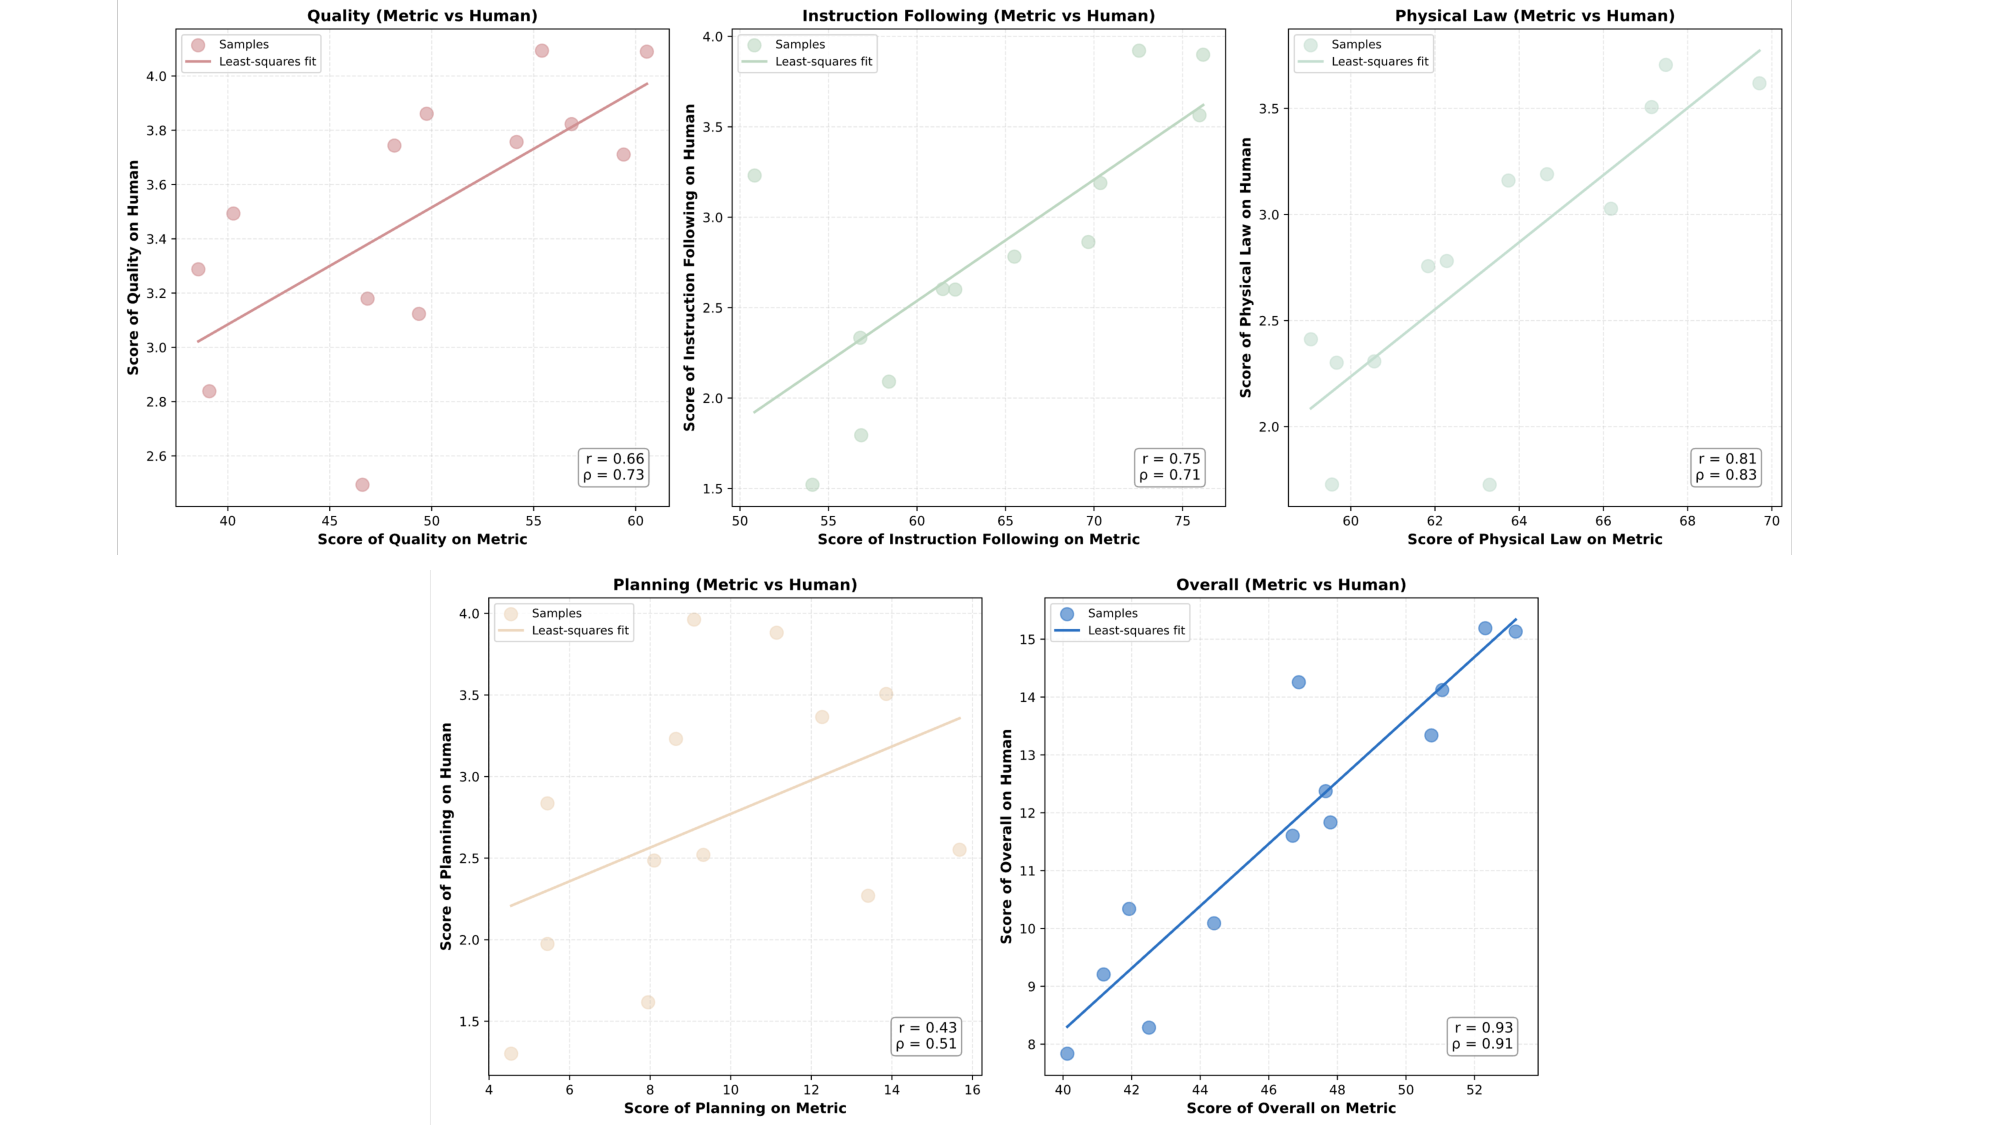
\includegraphics[width=1.0\textwidth]{figs/all_correlation.pdf} 
  \caption{\textbf{All correlation for WoW-World-Eval and Human Preference.} }
  \label{fig:all_correlation}
\end{figure*}

In section~\ref{ssec:quantitative}, we report the correlation between our overall scores and overall human preferences. However, to quantify how well WoW-World-Eval reflects human perception in all perspectives, we also provide the correlation between these four metrics—Video Quality, Instruction Understanding, Physical Law, and Planning. Figure~\ref{fig:all_correlation} reports both strong Pearson (r) and Spearman ($\rho$) correlations between all groups of benchmark scores and human preferences, which, importantly, confirms that metric-based evaluation can reliably approximate human judgment, supporting the use of WoW-World-Eval as a scalable alternative to costly human evaluations.

\paragraph{Video Quality.}
Quality metrics exhibit a quite strong correlation with human assessments (r = 0.66, $\rho$ = 0.73). This confirms that perceptual sharpness, temporal consistency, and high-level structure—captured jointly by FVD, PSNR, SSIM, DINO, and DreamSim—align well with how humans evaluate visual sensitivity.

\paragraph{Instruction Understanding.}
The Instruction Understanding score shows robust alignment with human preferences (r = 0.75, $\rho$ = 0.71). Models that accurately capture state transitions, object–action relationships, and multi-step task semantics tend to be judged by humans as better at “following instructions,” validating our caption-, sequence- and execution-based IU metrics.

\paragraph{Physical Law.}
Correlation is highest for Physical Law (r = 0.81, $\rho$ = 0.83). This indicates that humans are highly sensitive to violations of physics—object irregular motion, penetration, trajectory discontinuities, implausible state changes—and that our physics metrics effectively capture such failures. 

\paragraph{Planning.}
Planning demonstrates only moderate correlation with human ratings (r = 0.43, $\rho$ = 0.51). This reflects the inherent difficulty of automatically evaluating long-horizon reasoning and structured action sequences, as well as the limited planning ability of current video models. 

\subsection{Ground-truth video replay of IDM}
\label{ssec:IDM}
To ensure that our Inverse Dynamics Model (IDM) provides reliable supervision in the IDM Turing Test, we first validate the accuracy of a reproduced Gripper-Centric IDM (GC-IDM) following WoW~\cite{chi2025wow}. Before applying the IDM to model-generated videos, it is essential to verify that its action inference is sufficiently accurate on ground-truth real-world data; otherwise, low execution accuracy could stem from model weakness rather than the generated video being physically unrealistic.

We therefore evaluate GC-IDM across 9 manipulation tasks, each with 10 ground-truth execution videos. They are Easy (Pick bread and place on the plate; Close the drawer; Move the milk in front of the cup), Medium (Pick bread and place it in the upper drawer; Take the cup off the cup holder; Open the drawer) and Hard (Flip the button to the correct position; Hang the cup on the cup holder; Insert chopsticks into the bamboo tube). For each trial, we feed the real video sequence into GC-IDM, infer the corresponding gripper-centric action sequence, and replay it in the real world to measure Replay Execution Accuracy. As shown in Table~\ref{tab:relpay_results}, we showcased four of the tasks, GC-IDM substantially outperforms standard baselines such as ResNet-based inverse dynamics model and AVDC~\cite{Ko2023Learning} across all tasks, achieving an overall replay accuracy of 90\%, demonstrating strong fidelity in mapping real videos to executable actions. Representative frames from ground-truth video replays are provided in Figure~\ref{fig:real-world}.

This high replay accuracy confirms that GC-IDM is a reliable evaluator of physical plausibility. Consequently, when GC-IDM fails on model-generated videos, we can attribute the failure to deficiencies in video realism rather than inaccuracies in the IDM itself.

\begin{table}[h!]
\centering
\caption{\textbf{Comparison of Success Rate (\%) on various tasks across different models on ground-truth video replay.}}
\label{tab:relpay_results}
\resizebox{\linewidth}{!}{%
\begin{tabular}{@{\hskip 5pt}l@{\hskip 5pt} @{\hskip 5pt}cccc@{\hskip 5pt}}
\toprule
% \rowcolor{gray!15}
\textbf{Model / Task} & \textbf{Bread to Plate} & \textbf{Close Drawer} & \textbf{Move Milk} & \textbf{Bread in Drawer} \\
\midrule
\textbf{ResNet-MLPs}     & 6/10 & 7/10 & 5/10 & 4/10  \\
\textbf{AVDC}~\cite{Ko2023Learning}        & 3/10 & 4/10 & 4/10 & 2/10 \\
% Anypos~\citep{tan2025anypos}        & 8/10 & 9/10 & 8/10 & 7/10 & 6/10 & 3/10 & 2/15 & 2/15 & 0/15 \\
% 2DtrackerIDM        & 8/10 & 10/10 & 8/10 & 8/10 & 5/10 & 4/10 & 3/15 & 3/15 & 1/15 \\
\rowcolor{mylightgreen}
\textbf{GC-IDM}~\cite{chi2025wow}   & \textbf{10/10} & \textbf{9/10} & \textbf{9/10} & \textbf{8/10} \\
\bottomrule
\end{tabular}
}
\end{table}

\begin{figure*}[!h]
  \centering
  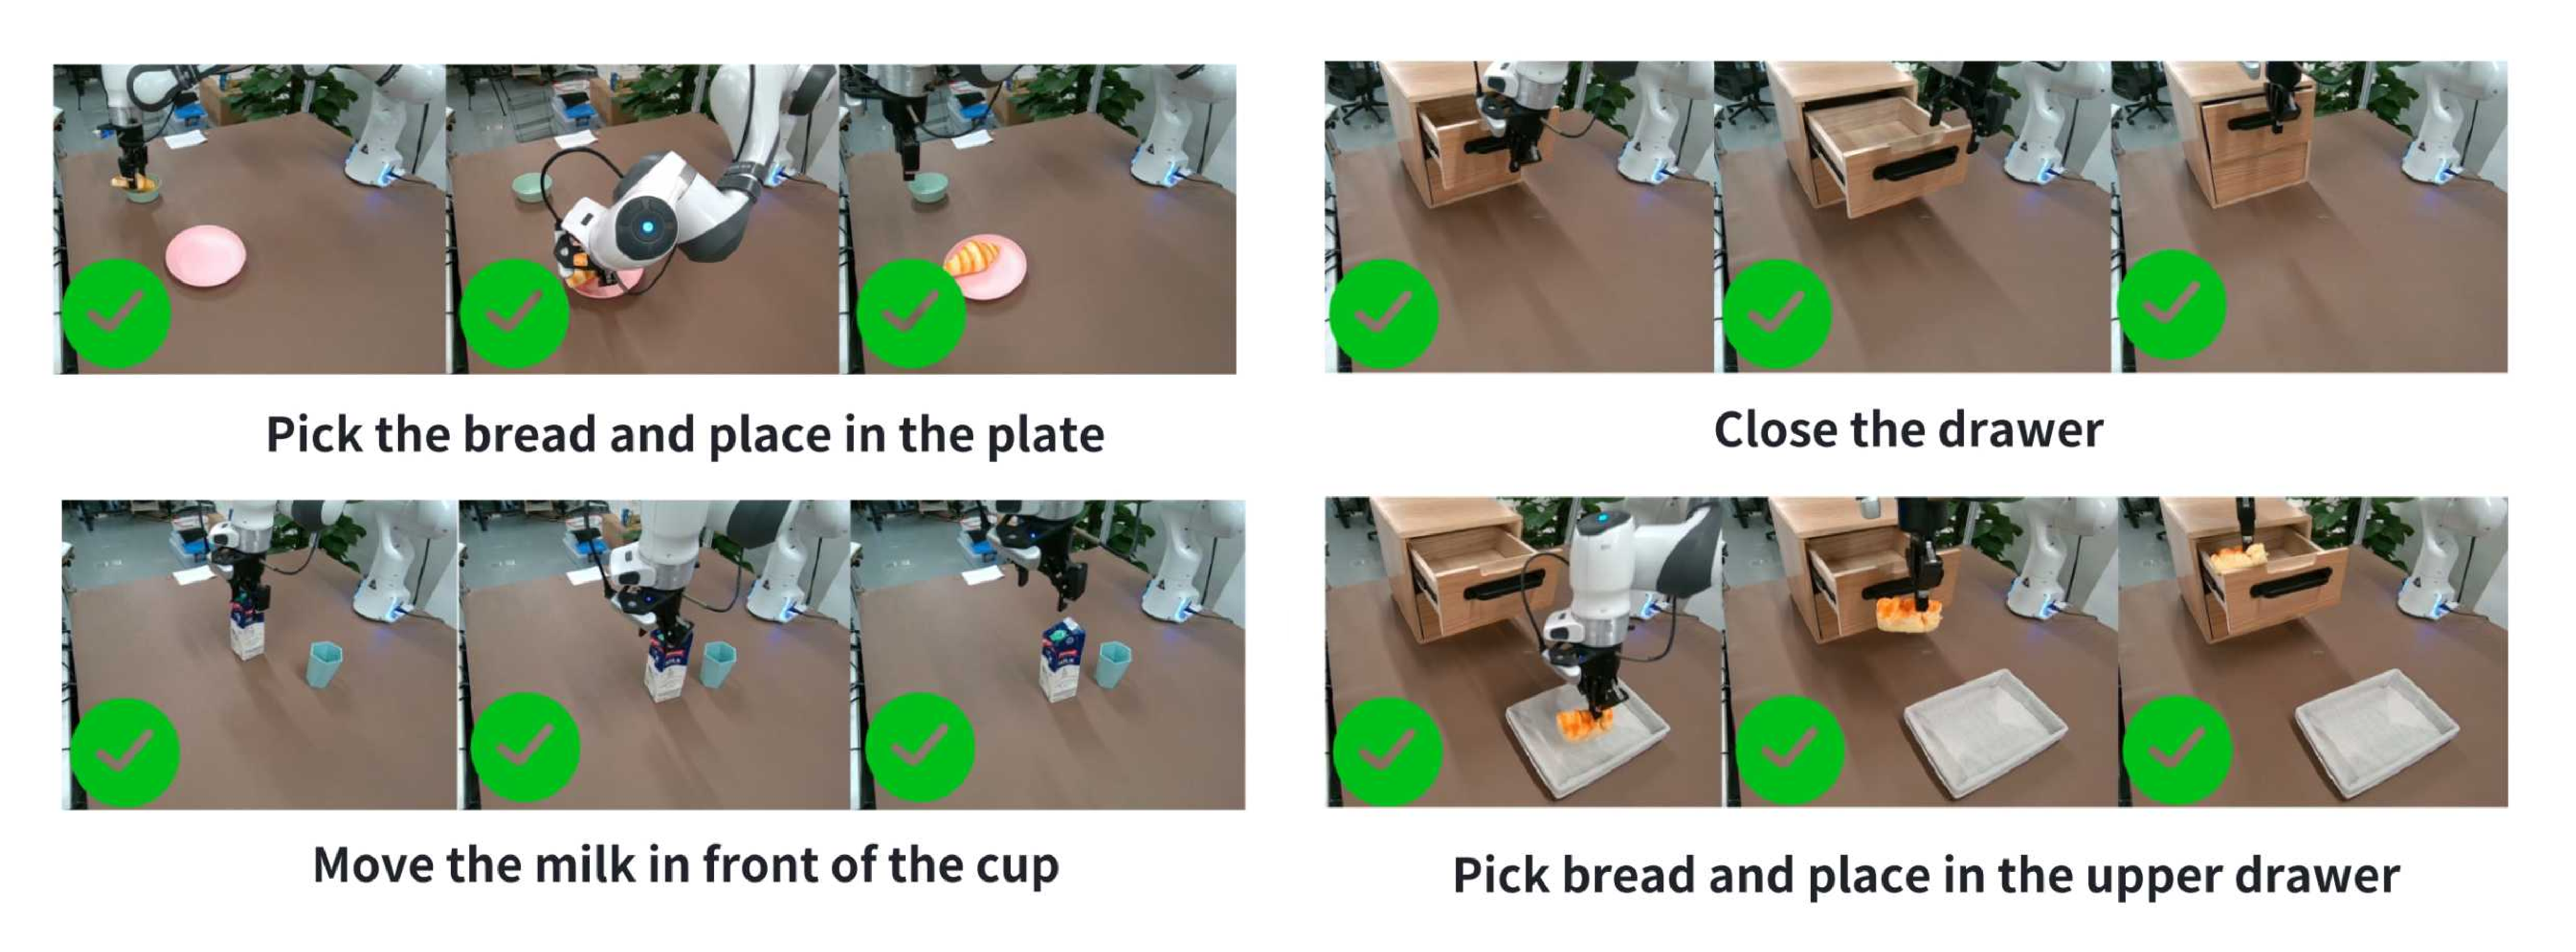
\includegraphics[width=1.0\textwidth]{figs/real-world.pdf} 
  \caption{\textbf{Real-World ground-truth video replay on real robot.} }
  \label{fig:real-world}
\end{figure*}

% \subsection{IDM Turing Test Detailed Results}
% \begin{table*}[h!]
% \centering
% \caption{\textbf{Detailed Comparison of Success Rate (\%) on various tasks across different models for IDM Turing Test.}}
% \label{tab:vla_results}
% \resizebox{\linewidth}{!}{%
% \begin{tabular}{@{\hskip 5pt}l@{\hskip 5pt} @{\hskip 5pt}cccc@{\hskip 5pt}}
% \toprule
% % \rowcolor{gray!15}
% \textbf{Model / Task} & \textbf{Bread to Plate} & \textbf{Close Drawer} & \textbf{Move Milk} & \textbf{Bread in Drawer}\\
% \midrule
% \textbf{Kling} & 3/9 & 0/9 & 5/9 & 0/9 \\
% \textbf{Hailuo} & 1/9 & 1/9 & 0/9 & 0/9 \\
% \textbf{CogVideoX/Cosmos-Predict1/Wan2.1} & 0/9 & 0/9 & 0/9 & 0/9 \\
% \textbf{Cosmos-Predict2} & 4/9 & 2/9 & 0/9 & 1/9 \\
% \rowcolor{mylightgreen}
% \textbf{WoW-wan} & \textbf{9/9} & \textbf{5/9} & \textbf{7/9} & \textbf{5/9}  \\
% \textbf{WoW-cosmos2} & 8/9 & 3/9 & 1/9 & 3/9 \\
% \bottomrule
% \end{tabular}
% }
% \end{table*}

\section{Case Results Visualization}
\label{sec:more_visualizations}
We also collect more generated results of different models for comparision, as visualized in Figure~\ref{fig:visualization2}, ~\ref{fig:visualization3}, ~\ref{fig:visualization4}.
\begin{figure*}[!h]
  \centering
  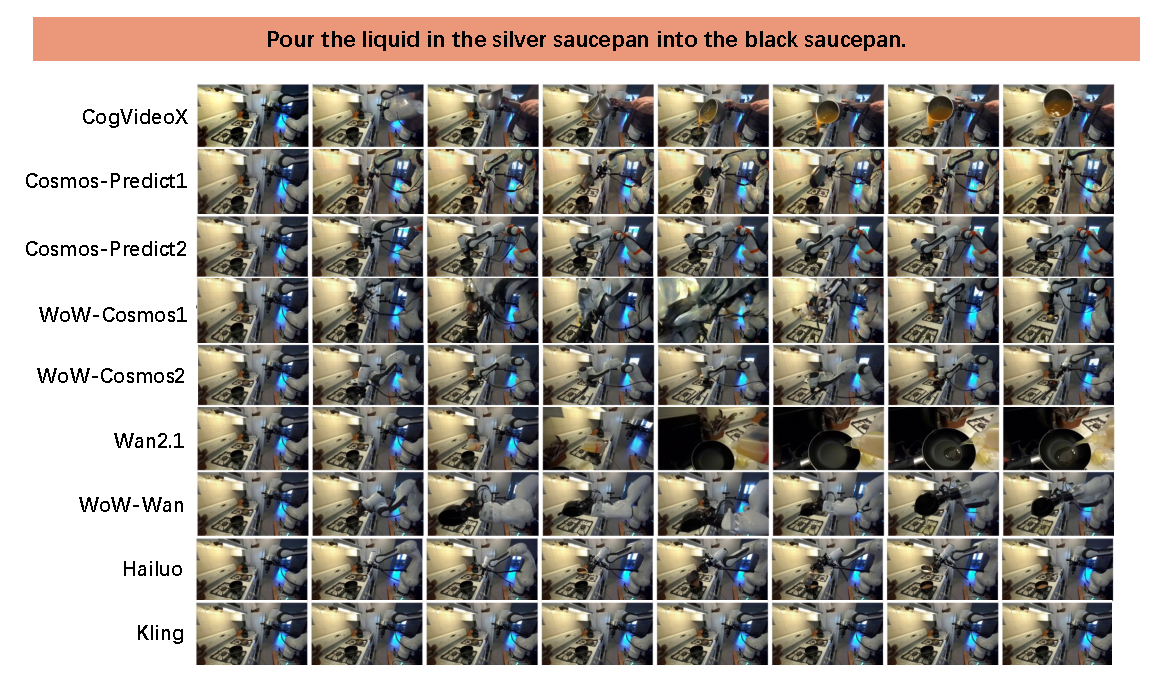
\includegraphics[width=1.0\textwidth]{figs/visualization2.pdf} 
  \caption{\textbf{More Case Visualization in Perception.} }
  \label{fig:visualization2}
\end{figure*}

\begin{figure*}[!h]
  \centering
  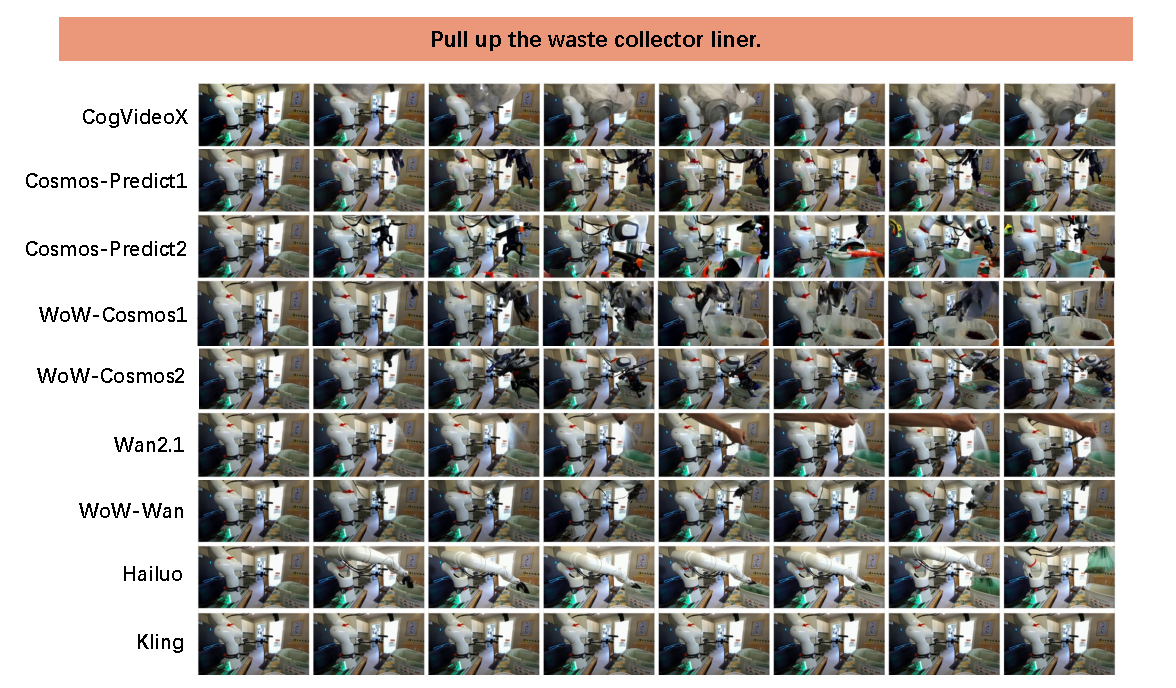
\includegraphics[width=1.0\textwidth]{figs/visualization3.pdf} 
  \caption{\textbf{More Case Visualization in Prediction.} }
  \label{fig:visualization3}
\end{figure*}

\begin{figure*}[!h]
  \centering
  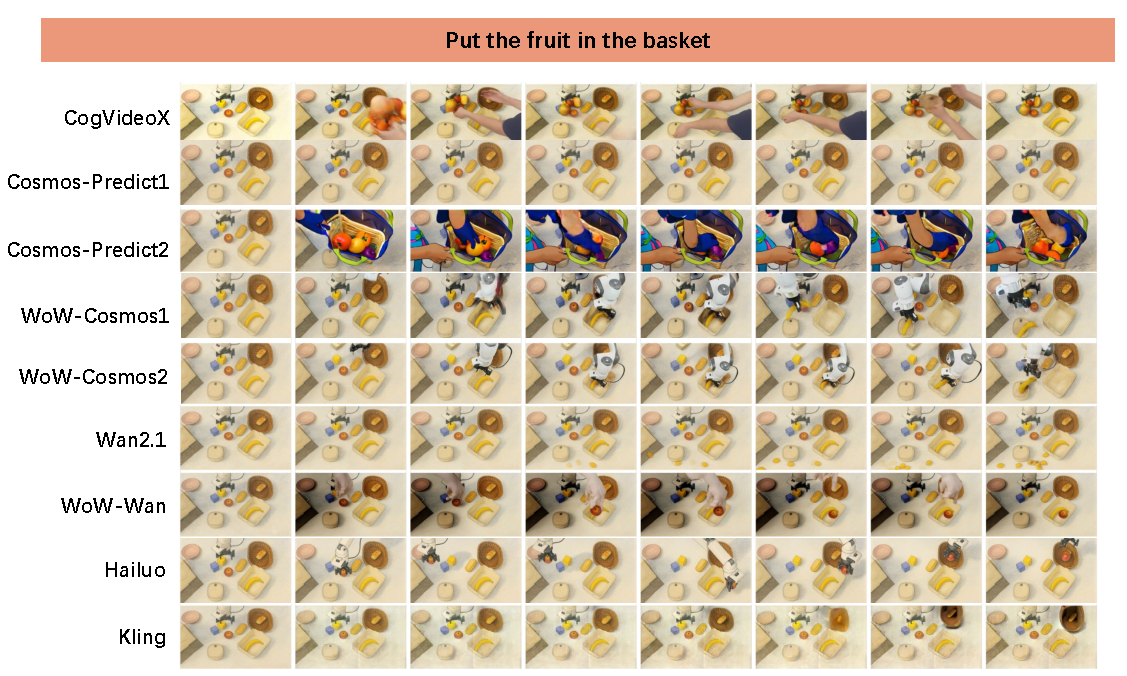
\includegraphics[width=1.0\textwidth]{figs/visualization4.pdf} 
  \caption{\textbf{More Case Visualization in Generalization.} }
  \label{fig:visualization4}
\end{figure*}

\section{Prompts}
For the prompts that we used in GPT for evaluation and data selection, or our own trained Physical MLLM.


\tcbset{
  promptstyle/.style={
    % enhanced,
    % % 边框颜色和粗细
    % frame=none,
    % % frame hidden,
    % % 填充背景色：设置为浅黄色 (e.g., yellow!15)
    % % 您可以根据需要调整百分比 (如 10, 15, 20) 来控制深浅。
    % colback=yellow!15, 
    % % 内部边距
    % boxsep=5pt,
    % % 盒子内边距
    % left=10pt,
    % right=10pt,
    % top=10pt,
    % bottom=10pt,
    % % 盒子不会断页
    % breakable,
    colback=yellow!15,    % 背景色
    colframe=yellow!15,   % 边框同色 = 看起来无边框
    boxrule=0pt,          % 去掉边框线条
    left=10pt,
    right=10pt,
    top=10pt,
    bottom=10pt,
    boxsep=5pt,
  }
}

% \clearpage
% \begin{strip}

\centering

% 确保 tcolorbox 占据全部宽度
\begin{tcolorbox}[
    %  promptstyle 且 colback=yellow!15
    promptstyle, 
    width=\linewidth, 
    breakable
    % breakable=true 
] 
    \subsection*{GPT Data Selection Prompt}

    \begin{lstlisting}[
        language=Tex, 
        basicstyle=\small\ttfamily,
        breaklines=true,
        frame=none, 
        columns=fullflexible,
        backgroundcolor=\color{yellow!15}, 
    ]
You are a robotics data selection and instruction rewriting assistant.
Input: one task instruction (text) and one first-frame image.
Output: JSON only, describing which data dimensions this sample belongs to, with evidence, confidence scores, and a rewritten instruction only for Perception dimensions.

Absolute Rules

Use only what is visible in the first frame and what is stated in the instruction. Do not hallucinate or import outside knowledge.

A dimension is valid only if:

The image provides clear visual evidence, and

The original instruction can be unambiguously rewritten (if Perception) or directly preserved (if Prediction/Planning).

If evidence is insufficient or ambiguous, do not assign the dimension; instead, explain in issues.

Multiple dimensions can be assigned; each must include its own score and evidence.

Instruction rewriting requirement:

Perception including rewrite instruction into an equivalent form using attributes / functions / spatial relations / affordances.

Prediction and Planning will always keep the original instruction unchanged.

Dimension Checklist
A. Perception

object-centric / object-attribute (color, number, shape, size, type)
    Paths must follow the format:
    'Perception/object-centric/object-attribute/color'
    'Perception/object-centric/object-attribute/type'
    etc.

Rewrite into attribute-based description.

object-centric / object-function

Rewrite into function-based description.

scene-centric / spatial-relation

Rewrite into relation-based description.

affordance-centric / object-affordance

Rewrite into affordance-based description.

B. Prediction

camera-view including no-occlude | semi-occlude.

physical-interaction including single-object/rigid | single-object/fluid | single-object/deformable | single-object/articulated | multi-object/rigid-rigid | multi-object/rigid-fluid | multi-object/rigid-deformable | multi-object/fluid-fluid | dual-arm-cooperate 

corner-case.

Keep original instruction (no rewriting).

C. Planning

long-term-instruction.

Keep original instruction (no rewriting).

JSON Output Format
{
  "input_instruction": "<original instruction>",
  "dimensions": [
    {
      "path": "Perception/object-centric/object-attribute/color",
      "score": 0.9,
      "evidence": "blue plate, red tomato, yellow pepper visible",
      "rewrite": "move the red and yellow objects to the blue object"
    },
    {
      "path": "Prediction/camera-view",
      "score": 0.8,
      "evidence": "all target objects fully visible",
      "rewrite": "keep original instruction"
    }
  ],
  "prediction": {
    "camera-view": {
      "label": "no-occlude | semi-occlude | unknown",
      "evidence": "<short evidence>",
      "score": 0.0
    },
    "physical-interaction": [
      {
        "label": "single-object/rigid | ...",
        "evidence": "<short evidence>",
        "score": 0.0
      }
    ]
  },
  "planning": [
    {
      "label": "long-term-instruction",
      "evidence": "<short evidence>",
      "score": 0.0,
      "rewrite": "keep original instruction"
    }
  ],
  "issues": [
    "<if there is missing evidence or ambiguity, explain here>"
  ]
}


For Perception dimensions, rewrite contains the modified instruction.

For Prediction and Planning dimensions, rewrite must be exactly "keep original instruction".

score is confidence for 0 to 1.

evidence is short, factual, visual clues only.

**Example**

Input:

instruction: move tomato and pepper to the plate

image: blue plate, red tomato, yellow pepper; no occlusion.

Output:

{
  "input_instruction": "move tomato and pepper to the plate",
  "dimensions": [
    {
      "path": "Perception/object-centric/object-attribute/color",
      "score": 0.95,
      "evidence": "blue plate; red tomato; yellow pepper visible",
      "rewrite": "move the red and yellow objects to the blue object"
    },
    {
      "path": "Prediction/camera-view",
      "score": 0.9,
      "evidence": "all target objects fully visible",
      "rewrite": "keep original instruction"
    }
  ],
  "prediction": {
    "camera-view": {
      "label": "no-occlude",
      "evidence": "all objects clearly visible",
      "score": 0.9
    },
    "physical-interaction": [
      {
        "label": "single-object/rigid",
        "evidence": "rigid tabletop objects",
        "score": 0.8
      }
    ]
  },
  "planning": [],
  "issues": []
}
    \end{lstlisting}
    
\end{tcolorbox}

\centering

% 确保 tcolorbox 占据全部宽度
\begin{tcolorbox}[
    %  promptstyle 且 colback=yellow!15
    promptstyle, 
    width=\linewidth, 
    breakable
    % breakable=true 
] 
    \subsection*{Instruction Semantic Correctness: Extract Video Semantic Caption}

    \begin{lstlisting}[
        language=Tex, 
        basicstyle=\small\ttfamily,
        breaklines=true,
        frame=none, 
        columns=fullflexible,
        backgroundcolor=\color{yellow!15}, 
    ]
Please analyze the instruction that I used to guide the model to generate video and the content of the following groundtruth video(there maybe no groundtruth video, if so please use only the instruction), extract semantic descriptions related to the robot's behavior. Focus on the following five aspects and provide one clear, concise sentence for each:
1. Initial State: The state of the object(s) and environment before any action (e.g., position, posture, quantity)
2. Processing State: The interaction process while the robot arm is operating (e.g., how it moves or manipulates the object)
3. Final State: The outcome after the action (e.g., new position or state of the object, whether the task goal was achieved)
4. Action: The main type of operation performed (e.g., grasping, pushing, placing)
5. Object: The object being manipulated (e.g., its color, shape, category)

Please output your result in the following format:
```
Initial State: ...
Processing State: ...
Final State: ...
Action: ...
Object: ...
```

Guidelines:
- Keep each sentence objective, specific, and based only on what is visible in the video.
- Do not add assumptions or imagined information.
- If any aspect is unclear or not visible, write "Unknown" for that field.
- Avoid overly abstract descriptions such as "successfully completed the task."

    \end{lstlisting}
    
\end{tcolorbox}

\centering

% 确保 tcolorbox 占据全部宽度
\begin{tcolorbox}[
    %  promptstyle 且 colback=yellow!15
    promptstyle, 
    width=\linewidth, 
    breakable
    % breakable=true 
] 
    \subsection*{Instruction Semantic Correctness: Compare Video Semantic Caption}

    \begin{lstlisting}[
        language=Tex, 
        basicstyle=\small\ttfamily,
        breaklines=true,
        frame=none, 
        columns=fullflexible,
        backgroundcolor=\color{yellow!15}, 
    ]
You are given structured semantic captions from two videos: the original ground truth and a generated version. Compare them across the following five dimensions and evaluate their semantic consistency.
"comparison_dimensions": {    
    "initial_state": "The object/environment status before any action",
    "processing_state": "How the robot interacts with the object during operation", 
    "final_state": "The outcome or resulting object state",
    "action": "The type of manipulation performed",
    "object": "The object being manipulated"
},
"scoring_guidelines": {
    "level_1": {
        "score": 1,
        "description": "Fully Consistent, Descriptions convey the same semantic content with only stylistic or wording differences"    
    },
    "level_2": {
        "score": 0.5,
        "description": "Partially Consistent, Descriptions differ in minor semantic details or omit secondary information, but task intent remains aligned"
    },
    "level_3": {
        "score": 0,
        "description": "Inconsistent, Descriptions conflict semantically, refer to different actions, goals, or object properties"
    }
},
"output_format": {
    "initial_state": "Score = [0 / 0.5 / 1] - Reason: ...",
    "processing_state": "Score = [0 / 0.5 / 1] - Reason: ...", 
    "final_state": "Score = [0 / 0.5 / 1] - Reason: ...",
    "action": "Score = [0 / 0.5 / 1] - Reason: ...",
    "object": "Score = [0 / 0.5 / 1] - Reason: ...",
    "overall": "Score = [0 / 0.5 / 1] - Summary Reason: ..."
},
"evaluation_principles": [
"Focus strictly on the semantic content of the captions, do not infer or assume actions or states that are not explicitly stated.",
"The overall score may reflect the average of the five dimensions, but should also consider whether the task intent and outcome remain semantically aligned."
]
Ground truth video caption is: {ground_truth_caption}
Generated video caption is: {generated_caption}
    \end{lstlisting}
    
\end{tcolorbox}

\centering

% 确保 tcolorbox 占据全部宽度
\begin{tcolorbox}[
    %  promptstyle 且 colback=yellow!15
    promptstyle, 
    width=\linewidth, 
    breakable
    % breakable=true 
] 
    \subsection*{Instruction Semantic Correctness: Evaluate Video Action Execution}

    \begin{lstlisting}[
        language=Tex, 
        basicstyle=\small\ttfamily,
        breaklines=true,
        frame=none, 
        columns=fullflexible,
        backgroundcolor=\color{yellow!15}, 
    ]
You are given a language instruction describing a series of robot manipulation actions, and a generated video that attempts to follow that instruction.
Your task has two parts:
PART 1: Action Sequence Consistency (Proportional Scoring)
Parse the instruction and extract the intended object-action pairs in order.
Analyze the generated video to determine the actual order of the executed object-action pairs. Compare the two sequences and compute a sequence match score:
    Sequence Match Scoring: 
        Score = (number of matching object-action pairs in correct order) / (total number of instruction pairs)
        Matching means: the object-action pair appears in the video and in the same relative order as in the instruction. Partial matches or out-of-order actions reduce the score.
    Output format:
        Instruction Sequence: [(object1, action1), (object2, action2), ...]
        Video Sequence: [(object1, action1), (object2, action2), ...]
        Sequence Match Score: X.XX (range: 0.00-1.00) - Reason: ...
        
PART 2: Action Execution Quality (Numerical Evaluation)
For each (object, action) pair in the instruction, evaluate execution quality using a 1-5 numerical scale:
    Execution Quality Scoring:
        1 - Object did not move AND action was not attempted
        2 - Object moved slightly OR action was partially attempted
        3 - Object moved slightly AND action was partially attempted
        4 - Object reached target state OR action completed successfully
        5 - Object reached target state AND action completed successfully

    Base this strictly on visible evidence in the video. Be conservative in scoring.

    Output format:
        Execution Quality:
        - (object1, action1): Score = [1-5] - Reason: ...
        - (object2, action2): Score = [1-5] - Reason: ...
        
Final Combined Output:
    Instruction Sequence: ...
    Video Sequence: ...
    Sequence Match Score: X.XX (range: 0.00-1.00) - Reason: ...
    Execution Quality:
    - (object1, action1): Score = [1-5] - Reason: ...
    - (object2, action2): Score = [1-5] - Reason: ...
    Instruction is: {instruction}

    \end{lstlisting}
    
\end{tcolorbox}


\centering
\begin{tcolorbox}[
    %  promptstyle 且 colback=yellow!15
    promptstyle, 
    width=\linewidth, 
    breakable 
] 
    \subsection*{Physical Common Sense: Stage 2: Scoring Alignment Fine-tuning Prompt }

    \begin{lstlisting}[
        language=Tex, 
        basicstyle=\small\ttfamily,
        breaklines=true,
        frame=none, 
        columns=fullflexible,
        backgroundcolor=\color{yellow!15}, 
    ]
You are an expert AI video evaluator. Your task is to analyze the provided video, which was generated from the accompanying text prompt. You must score the video on a scale of 1 to 5 across four dimensions based on the precise criteria listed below.

Evaluation Criteria:

1. Video Quality (1-5):

    5: Clear, stable, natural colors, no generation artifacts.

    4: Minor flaws (e.g., occasional flicker, slight blur) that don't detract from the overall view.

    3: Noticeable flaws (e.g., persistent noise, subject out of focus) but core content is understandable.

    2: Severe defects (e.g., unstable subject form, heavy jitter) that significantly impair understanding.

    1: Extremely poor quality, making the subject or content unrecognizable.

2. Instruction Following (1-5):

    5: Perfectly matches the prompt; all core elements and details are accurately represented.

    4: Core elements are correct, but a minor detail (e.g., color, location) is missed or incorrect.

    3: The core element (subject or action) deviates significantly but is still partially related to the prompt.

    2: The core element is fundamentally misinterpreted; the content is seriously inconsistent with the prompt.

    1: Completely unrelated to the prompt; a random generation.

3. Physical Consistency (1-5):

    5: Fully consistent with physics; interactions are believable, no object clipping or floating.

    4: A momentary, almost unnoticeable physical anomaly (e.g., slight clipping) that doesn't affect the task.

    3: A noticeable physical error (e.g., arm passes through a table) that doesn't break the core task logic.

    2: A severe physical error that causes the task to fail or its logic to break (e.g., a hand passes through the target object).

    1: A complete lack of physical logic; chaotic and disorderly interactions.

4. Planning Logic (1-5):

    5: The plan is logical, efficient, with no redundant actions, and successfully achieves the goal.

    4: The plan is effective and successful but contains minor redundant or inefficient movements.

    3: The goal is achieved, but the process is convoluted or clumsy; the plan is illogical.

    2: The plan has critical errors or missing steps, leading to task failure.

    1: Actions are random and chaotic, with no discernible goal or plan.

Analyze the following inputs:

Original Prompt: {instruction}
Generated Video: <video>
Your final answer must be a single, valid JSON object and nothing else. Do not include any explanations, conversational text, or markdown formatting around the JSON block.
Your JSON Answer:
{
  "video_quality": <integer_score>,
  "instruction_following": <integer_score>,
  "physical_consistency": <integer_score>,
  "planning_logic": <integer_score>
}
    \end{lstlisting}
    
\end{tcolorbox}

% \end{strip}




% \begin{strip}
\centering

% 确保 tcolorbox 占据全部宽度
\begin{tcolorbox}[
    %  promptstyle 且 colback=yellow!15
    promptstyle, 
    width=\linewidth, 
    breakable
    % breakable=true 
] 
    \subsection*{Physical Common Sense: 6-Dimension Evaluation Prompt}

    \begin{lstlisting}[
        language=Tex, 
        basicstyle=\small\ttfamily,
        breaklines=true,
        frame=none, 
        columns=fullflexible,
        backgroundcolor=\color{yellow!15}, 
    ]
Please evaluate the following video strictly based on whether it follows real-world physics laws.
This is not a test of whether it is AI-generated, but only judge its physical plausibility.
Scoring System (1 to 5 scale):
For each of the six categories below, assign a score from 1 to 5:
5 = Fully consistent with real-world physics
4 = Mostly consistent, only small flaws
3 = Partially consistent, with some clear issues
2 = Often inconsistent, unrealistic in multiple ways
1 = Clearly violates physical laws
- null = Not applicable (no relevant content in video)
For each of the following categories:
- Give a score (1 to 5) or null if the category does not appear at all in the video
- Provide a brief explanation (1 to 2 sentences) for each score
Return your output in structured JSON as shown below.

---
Evaluation Criteria (Detailed):
1. Object Interaction and State Changes
  - Do objects respond naturally when they touch, collide, bounce, break, or are pushed/pulled?
  - Is there a realistic cause-and-effect in object contact?
  - Do interactions follow Newton's laws (e.g., action/reaction, inertia)?
  - Are deformations (e.g., squashing, bending) consistent with materials?
  - Do objects maintain consistent color, quantity, shape, and size throughout interactions?
2. Basic Physical Properties
  - Does gravity act in the correct direction and magnitude (e.g., falling speed)?
  - Is there realistic motion under inertia and deceleration?
  - Does friction behave naturally (e.g., sliding slows over time)?
  - Are materials (heavy/light) behaving correctly based on mass or density?
3. Temporal and Causal Consistency
  - Do effects follow causes in the right order and with realistic timing?
  - Are there appropriate delays in mechanical systems, collisions, or triggered motions?
  - Is there a consistent flow of time across all elements (e.g., no time jumps or impossible overlaps)?
4. Lighting, Shadows, and Reflections
  - Are shadows cast in the correct direction and shape relative to light sources?
  - Is there consistent lighting across surfaces and objects?
  - Do reflective surfaces (mirrors, metal, water) behave correctly based on angles?
  - Is light intensity and falloff physically accurate (not flat or overly uniform)?
5. Fluid and Particle Behavior
  - Do water, smoke, fire, or dust behave according to fluid dynamics?
  - Is there natural turbulence, diffusion, and randomness?
  - Do particles (like debris, sparks, splashes) move in a physically plausible way?
  - Is there appropriate interaction with solid surfaces (e.g., splashes bounce, smoke drifts)?
6. Local Anomalies or Violations
  - Are there any visual inconsistencies like:
    - sudden object movement without cause
    - teleportation or disappearing items
    - objects passing through others (no collision)
    - animation glitches, floating artifacts, or broken motion?
  - Do all parts of the scene stay consistent frame to frame?
---
Return your output in structured JSON as shown below.
    - object_interaction: {score: int|null, comment: str}
    - physical_properties: {score: int|null, comment: str}
    - temporal_consistency: {score: int|null, comment: str}
    - lighting_and_reflections: {score: int|null, comment: str}
    - fluids_and_particles: {score: int|null, comment: str}
    - local_anomalies: {score: int|null, comment: str}
    \end{lstlisting}
    
\end{tcolorbox}

% \end{strip}

\centering

% 确保 tcolorbox 占据全部宽度
\begin{tcolorbox}[
    %  promptstyle 且 colback=yellow!15
    promptstyle, 
    width=\linewidth, 
    breakable
    % breakable=true 
] 
    \subsection*{Dense Prompts Extension Prompt}

    \begin{lstlisting}[
        language=Tex, 
        basicstyle=\small\ttfamily,
        breaklines=true,
        frame=none, 
        columns=fullflexible,
        backgroundcolor=\color{yellow!15}, 
    ]
You are an expert in Embodied AI tasked with generating dense and standardized textual descriptions of robot episodes. Your goal is to re-caption a brief, potentially ambiguous, episode description  into a richer, more precise narrative,but no more than 150 words. This serves two main purposes:
1.  To clarify ambiguous action descriptions with precise technical terminology.
2.  To unify the textual representation of similar actions across different datasets, ensuring consistency in phrasing and detail.

When generating the dense caption, adhere to the following structure and include these specific details:

1.  **Overall Scene & Goal Overview:**
    *   Begin with a concise summary of the robot's primary goal or the main action being performed in the scene, directly derived or inferred from the input .

2.  **Environment Description:**
    *   Describe the robot's operational environment (e.g., kitchen, laboratory, office, cluttered tabletop, outdoor path).
    *   Include relevant ambient conditions: lighting (e.g., bright, dim, natural, artificial), indoor/outdoor setting, and weather if applicable (e.g., sunny, overcast for outdoor scenes).

3.  **Robot Characteristics:**
    *   Specify key characteristics of the robot if inferable or if it's a common type in embodied AI (e.g., humanoid, mobile manipulator with a single arm, quadruped, drone).
    *   Note its general appearance if significant (e.g., color scheme, predominant material like metallic or plastic).
    *   Mention its gripper type if relevant to the action (e.g., parallel jaw gripper, suction cup, multi-finger dexterous hand).

4.  **Camera Perspective & Motion:**
    *   Detail the camera's perspective (e.g., first-person (egocentric/robot's POV), third-person fixed, third-person dynamic/following, eye-in-hand, overhead).
    *   Describe any significant camera movement (e.g., static, panning to follow action, smooth tracking shot, handheld jitter if applicable).

5.  **Robot Sub-goal & Granular Action Breakdown:**
    *   Infer and explicitly state the immediate sub-goal the robot is trying to achieve based on the input.
    *   Provide a granular breakdown of the robot's actions. Use precise, standardized technical action terminology (e.g., "Navigate_to [location]", "Perceive [object]", "Grasp [object]", "Lift [object]", "Move_arm_to [target_pose]", "Place [object] at [location]", "Release [object]", "Push [object]", "Rotate [object]").
    *   Clearly identify the object(s) being manipulated and any changes in their state or location.

6.  **Post-Action State:**
    *   Briefly describe the state of the robot and the key manipulated object(s) *after* the described action sequence is completed.

**Constraints:**
*   The final description should be dense, focusing on factual and observable details.
*   Aim for a total length of approximately 100-150 words.
*   Use consistent terminology for common actions and objects.
*   Avoid filler words or subjective stylistic descriptions not grounded in typical embodied AI contexts.
*   Only describe elements plausibly present or inferable from a typical embodied AI episode matching the `Given Input`. Do not invent fantastical details.
*   Never mention elements outside the implied scene or action.

---
**Example of Use:**

Let's say the given short episode description  is: "drop the apple in the bowl"

**Given Input :drop the apple in the bowl

**Your Dense Recaption (Output based on the prompt above):**

The robot's primary goal is to place an apple into a designated bowl.
The scene is set in a brightly lit kitchen environment, specifically on a clean countertop. The robot is a single-arm manipulator, predominantly white with grey joints, equipped with a parallel jaw gripper, likely mounted on a stationary or mobile base (partially visible). The camera is a static third-person view, positioned to offer a clear side-angle of the robot's arm and the workspace, including the target bowl.
The robot's sub-goal is to successfully deposit the apple. The action sequence begins with the robot's arm, already grasping a red apple, positioned directly above a ceramic bowl. The arm executes a 'Move_arm_to [bowl_center_above]' command, followed by a 'Lower_arm' motion. The gripper then performs a 'Release [apple]' action. Finally, the arm might execute a 'Retract_arm' motion away from the bowl.
After the action, the red apple rests inside the bowl on the countertop, and the robot's gripper is open and clear of the bowl.

Given Input : {instruction}
Your Dense Recaption:

    \end{lstlisting}
    
\end{tcolorbox}

\clearpage

% \section{Rationale}
% \label{sec:rationale}
% % 
% Having the supplementary compiled together with the main paper means that:
% % 
% \begin{itemize}
% \item The supplementary can back-reference sections of the main paper, for example, we can refer to \cref{sec:intro};
% \item The main paper can forward reference sub-sections within the supplementary explicitly (e.g., referring to a particular experiment); 
% \item When submitted to arXiv, the supplementary will already included at the end of the paper.
% \end{itemize}
% % 
% To split the supplementary pages from the main paper, you can use \href{https://support.apple.com/en-ca/guide/preview/prvw11793/mac#:~:text=Delete%20a%20page%20from%20a,or%20choose%20Edit%20%3E%20Delete).}{Preview (on macOS)}, \href{https://www.adobe.com/acrobat/how-to/delete-pages-from-pdf.html#:~:text=Choose%20%E2%80%9CTools%E2%80%9D%20%3E%20%E2%80%9COrganize,or%20pages%20from%20the%20file.}{Adobe Acrobat} (on all OSs), as well as \href{https://superuser.com/questions/517986/is-it-possible-to-delete-some-pages-of-a-pdf-document}{command line tools}.